\documentclass[12pt,letterpaper]{article}  
  
% ============================================================  
% PACKAGES  
% ============================================================  

% PACKAGES  
% ============================================================  
\usepackage[margin=1in]{geometry}  
\usepackage{amsmath,amssymb,amsfonts}  
\usepackage{listings}  
\usepackage{xcolor}  
\usepackage{hyperref}  
\usepackage{booktabs}  
\usepackage{longtable}  
\usepackage{array}  
\usepackage{graphicx}  
\usepackage{float}  
\usepackage{fancyhdr}  
\usepackage{titlesec}  
\usepackage{enumitem}  
\usepackage{mdframed}  
\usepackage{caption}  
\usepackage{subcaption}  
\usepackage{tikz}  
\usetikzlibrary{arrows.meta, positioning, shapes.geometric, fit, backgrounds}  
  
% ============================================================  
% COLORS  
% ============================================================  
\definecolor{fortranblue}{RGB}{0,70,140}  
\definecolor{fortrangreen}{RGB}{0,120,0}  
\definecolor{fortranred}{RGB}{160,0,0}  
\definecolor{fortranorange}{RGB}{200,100,0}  
\definecolor{codebg}{RGB}{248,248,248}  
\definecolor{framecolor}{RGB}{180,180,180}  
\definecolor{commentcolor}{RGB}{80,120,80}  
\definecolor{keywordcolor}{RGB}{0,0,180}  
\definecolor{stringcolor}{RGB}{160,0,0}  
\definecolor{highlightbg}{RGB}{255,255,200}  
\definecolor{sectioncolor}{RGB}{0,70,140}  
\definecolor{boxbg}{RGB}{240,248,255}  
\definecolor{boxframe}{RGB}{100,150,200}  
\definecolor{warnbg}{RGB}{255,248,230}  
\definecolor{warnframe}{RGB}{200,150,50}  
  
% ============================================================  
% LISTINGS STYLE  
% ============================================================  
\lstdefinelanguage{Fortran90KPP}{  
  language=[90]Fortran,  
  morekeywords={SUBROUTINE,END,IF,THEN,ELSE,ENDIF,DO,ENDDO,CALL,  
                RETURN,IMPLICIT,NONE,INTEGER,REAL,LOGICAL,CHARACTER,  
                PARAMETER,COMMON,INCLUDE,IFDEF,IFNDEF,ENDIF,DEFINE,  
                UNDEF,MIN,MAX,SQRT,ABS,SIGN,EXP,LOG,INT,FLOAT},  
  keywordstyle=\color{keywordcolor}\bfseries,  
  commentstyle=\color{commentcolor}\itshape,  
  stringstyle=\color{stringcolor},  
  basicstyle=\ttfamily\footnotesize,  
  backgroundcolor=\color{codebg},  
  frame=single,  
  framerule=0.8pt,  
  rulecolor=\color{framecolor},  
  numbers=left,  
  numberstyle=\tiny\color{gray},  
  numbersep=8pt,  
  breaklines=true,  
  breakatwhitespace=false,  
  tabsize=2,  
  showspaces=false,  
  showstringspaces=false,  
  captionpos=b,  
  xleftmargin=15pt,  
  xrightmargin=5pt,  
  aboveskip=8pt,  
  belowskip=8pt,  
  sensitive=false,  
  morecomment=[l]{!},  
  morecomment=[l]{c},  
  morecomment=[l]{C},  
  morecomment=[s]{/*}{*/},  
  morestring=[b]",  
  morestring=[b]',  
  escapeinside={(*@}{@*)}  
}  
  
\lstset{  
  language=Fortran90KPP,  
  style={}  
}  
  
% ============================================================  
% CUSTOM ENVIRONMENTS  
% ============================================================  
\newmdenv[  
  backgroundcolor=boxbg,  
  linecolor=boxframe,  
  linewidth=1.5pt,  
  roundcorner=4pt,  
  innerleftmargin=10pt,  
  innerrightmargin=10pt,  
  innertopmargin=8pt,  
  innerbottommargin=8pt  
]{infobox}  
  
\newmdenv[  
  backgroundcolor=warnbg,  
  linecolor=warnframe,  
  linewidth=1.5pt,  
  roundcorner=4pt,  
  innerleftmargin=10pt,  
  innerrightmargin=10pt,  
  innertopmargin=8pt,  
  innerbottommargin=8pt  
]{warnbox}  
  
\newmdenv[  
  backgroundcolor=codebg,  
  linecolor=framecolor,  
  linewidth=1pt,  
  roundcorner=2pt,  
  innerleftmargin=8pt,  
  innerrightmargin=8pt,  
  innertopmargin=6pt,  
  innerbottommargin=6pt  
]{codebox}  
  
% ============================================================  
% HEADER / FOOTER  
% ============================================================  
\pagestyle{fancy}  
\fancyhf{}  
\fancyhead[L]{\textcolor{sectioncolor}{\textbf{MITgcm KPP Package}}}  
\fancyhead[R]{\textcolor{gray}{\textit{Technical Reference}}}  
\fancyfoot[C]{\thepage}  
\renewcommand{\headrulewidth}{1pt}  
\renewcommand{\headrule}{\color{sectioncolor}\hrule width\headwidth height\headrulewidth}  
  
% ============================================================  
% SECTION FORMATTING  
% ============================================================  
\titleformat{\section}  
  {\color{sectioncolor}\Large\bfseries}  
  {\thesection}{1em}{}[\color{sectioncolor}\titlerule]  
  
\titleformat{\subsection}  
  {\color{fortranblue}\large\bfseries}  
  {\thesubsection}{1em}{}  
  
\titleformat{\subsubsection}  
  {\color{fortranblue}\normalsize\bfseries}  
  {\thesubsubsection}{1em}{}  
  
% ============================================================  
% HYPERREF SETUP  
% ============================================================  
\hypersetup{  
  colorlinks=true,  
  linkcolor=fortranblue,  
  citecolor=fortrangreen,  
  urlcolor=fortranred,  
  pdftitle={MITgcm KPP Package Technical Reference},  
  pdfauthor={Auto-generated from source analysis},  
  pdfsubject={Ocean vertical mixing parameterization}  
}  
  
% ============================================================  
% MATH OPERATORS  
% ============================================================  
\DeclareMathOperator{\sgn}{sgn}  
\newcommand{\hbl}{h_{\mathrm{bl}}}  
\newcommand{\ustar}{u_*}  
\newcommand{\Ri}{\mathrm{Ri}}  
\newcommand{\Ricr}{\mathrm{Ri_{cr}}}  
\newcommand{\KzT}{\kappa_T}  
\newcommand{\KzS}{\kappa_S}  
\newcommand{\Kzm}{\kappa_m}  
\newcommand{\wm}{w_m}  
\newcommand{\ws}{w_s}  
\newcommand{\ghat}{\hat{\gamma}}  
\newcommand{\bfsfc}{B_f}  
  
% ============================================================  
\begin{document}  
% ============================================================  
  
% ============================================================  
% TITLE PAGE  
% ============================================================  
\begin{titlepage}  
\begin{center}  
\vspace*{2cm}  
  
{\Huge\color{sectioncolor}\bfseries MITgcm KPP Package}\\[0.5cm]  
{\Large\color{fortranblue} K-Profile Parameterization for Vertical Ocean Mixing}\\[0.5cm]  
{\large\color{gray} Technical Reference: Architecture, Physics, and Implementation}  
  
\vspace{1.5cm}  
\rule{\linewidth}{2pt}  
\vspace{0.5cm}  
  
\begin{infobox}  
\textbf{Package Location:} \texttt{MITgcm/pkg/kpp/}\\[4pt]  
\textbf{Primary Reference:} Large, W.G., McWilliams, J.C., Doney, S.C. (1994).  
\textit{Oceanic vertical mixing: a review and a model with a nonlocal boundary layer  
parameterization}. Reviews of Geophysics, 32(4), 363--403.\\[4pt]  
\textbf{Additional Reference:} van Roekel et al.\ (2018). \textit{The KPP Boundary  
Layer Scheme for the Ocean: Revisiting Its Formulation and Benchmarking  
One-Dimensional Simulations Relative to LES}. JAMES, 10, 2647--2685.  
\end{infobox}  
  
\vspace{1cm}  
\rule{\linewidth}{1pt}  
\vspace{0.5cm}  
  
{\large\textbf{Compiled from source files:}}\\[6pt]  
\begin{tabular}{ll}  
\texttt{KPP.h}                  & State variable declarations \\  
\texttt{KPP\_OPTIONS.h}          & Compile-time options \\  
\texttt{KPP\_PARAMS.h}           & Run-time parameters \\  
\texttt{kpp\_calc.F}             & Main driver routine \\  
\texttt{kpp\_routines.F}         & Core physics subroutines \\  
\texttt{kpp\_forcing\_surf.F}    & Surface forcing preparation \\  
\texttt{kpp\_calc\_diff\_t.F}    & Temperature diffusivity interface \\  
\texttt{kpp\_calc\_diff\_s.F}    & Salinity diffusivity interface \\  
\texttt{kpp\_calc\_diff\_ptr.F}  & Passive tracer diffusivity interface \\  
\texttt{kpp\_calc\_visc.F}       & Viscosity interface \\  
\texttt{kpp\_transport\_t.F}     & Non-local temperature flux \\  
\texttt{kpp\_transport\_s.F}     & Non-local salinity flux \\  
\texttt{kpp\_transport\_ptr.F}   & Non-local passive tracer flux \\  
\texttt{kpp\_init\_fixed.F}      & Time-invariant initialization \\  
\texttt{kpp\_init\_varia.F}      & Time-varying initialization \\  
\texttt{kpp\_readparms.F}        & Parameter file reader \\  
\texttt{kpp\_output.F}           & Diagnostics and I/O \\  
\texttt{kpp\_check.F}            & Consistency checks \\  
\texttt{kpp\_do\_exch.F}         & Halo exchanges \\  
\texttt{kpp\_diagnostics\_init.F}& Diagnostics registration \\  
\end{tabular}  
  
\vfill  
{\color{gray}\today}  
\end{center}  
\end{titlepage}  
  
% ============================================================  
\tableofcontents  
\newpage  
% ============================================================  
  
% ============================================================  
\section{Introduction and Scientific Background}  
% ============================================================  
  
The K-Profile Parameterization (KPP) is a first-order turbulence closure  
scheme designed to represent vertical mixing throughout the full ocean  
water column. It was developed by Large, McWilliams, and Doney (1994;  
hereafter LMD94) and has become one of the most widely used vertical  
mixing parameterizations in ocean general circulation models. The MITgcm  
implementation closely follows LMD94 but has been adapted for the  
finite-volume, staggered-grid architecture of MITgcm.  
  
\subsection{Physical Motivation}  
  
Vertical mixing in the ocean is driven by several distinct physical  
mechanisms that operate in different parts of the water column:  
  
\begin{enumerate}[leftmargin=*, label=\textbf{\arabic*.}]  
  \item \textbf{Surface boundary layer turbulence} -- Wind stress and  
        surface buoyancy fluxes drive turbulent kinetic energy into the  
        ocean surface layer. This energy is distributed throughout the  
        oceanic planetary boundary layer (OBL) to depth $\hbl$.  
  
  \item \textbf{Shear instability} -- Vertical shear in the horizontal  
        velocity field can generate turbulence when the local Richardson  
        number falls below a critical threshold.  
  
  \item \textbf{Static instability / convection} -- Unstable density  
        stratification (dense water over light water) drives rapid  
        convective overturning.  
  
  \item \textbf{Internal wave breaking} -- Background internal wave  
        activity maintains a minimum level of mixing throughout the  
        interior ocean.  
  
  \item \textbf{Double diffusion} -- The differential molecular  
        diffusivities of heat and salt can give rise to salt fingering  
        and diffusive convection when the density ratio $R_\rho$ is near  
        unity.  
\end{enumerate}  
  
\subsection{Two-Region Decomposition}  
  
KPP divides the water column into two regions, each with its own mixing  
parameterization:  
  
\begin{infobox}  
\textbf{Region 1 -- Oceanic Boundary Layer} ($z > -\hbl$): \\  
Mixing is parameterized using a smooth turbulent velocity scale profile  
that depends on surface forcing, boundary layer depth, and stability.  
The profile is constrained to match interior mixing at $z = -\hbl$.  
A non-local (counter-gradient) transport term $\ghat$ is active under  
unstable (convective) forcing.\\[6pt]  
\textbf{Region 2 -- Ocean Interior} ($z < -\hbl$): \\  
Mixing depends on the local Richardson number for shear-driven  
instability, on the Brunt-V\"{a}is\"{a}l\"{a} frequency for  
convective instability, and includes a constant background contribution  
from internal wave breaking.  
\end{infobox}  
  
\subsection{Key State Variables}  
  
The KPP package maintains the following global state arrays, declared  
in \texttt{KPP.h}:  
  
\begin{longtable}{lp{2cm}p{6cm}l}  
\toprule  
\textbf{Variable} & \textbf{Dims} & \textbf{Description} & \textbf{Units} \\  
\midrule  
\endhead  
\texttt{KPPviscAz}  & $(x,y,N_r)$ & Vertical eddy viscosity & m$^2$/s \\  
\texttt{KPPdiffKzT} & $(x,y,N_r)$ & Vertical heat diffusivity & m$^2$/s \\  
\texttt{KPPdiffKzS} & $(x,y,N_r)$ & Vertical salt/tracer diffusivity & m$^2$/s \\  
\texttt{KPPghat}    & $(x,y,N_r)$ & Non-local transport coefficient & s/m$^2$ \\  
\texttt{KPPhbl}     & $(x,y)$     & Boundary layer depth & m \\  
\texttt{KPPfrac}    & $(x,y)$     & SW fraction heating mixed layer & -- \\  
\texttt{KPPplumefrac}& $(x,y)$   & Salt plume fraction penetrating OBL & -- \\  
\bottomrule  
\end{longtable}  
  
These arrays are computed by \texttt{KPP\_CALC} and subsequently consumed  
by the tracer and momentum advection--diffusion solvers each timestep.  
  
% ============================================================  
\section{Package Architecture and Call Flow}  
% ============================================================  
  
\subsection{Initialization Sequence}  
  
The KPP package initialization occurs in two stages, called during  
\texttt{INITIALISE\_FIXED} and \texttt{INITIALISE\_VARIA} respectively.  
  
\begin{figure}[H]  
\centering  
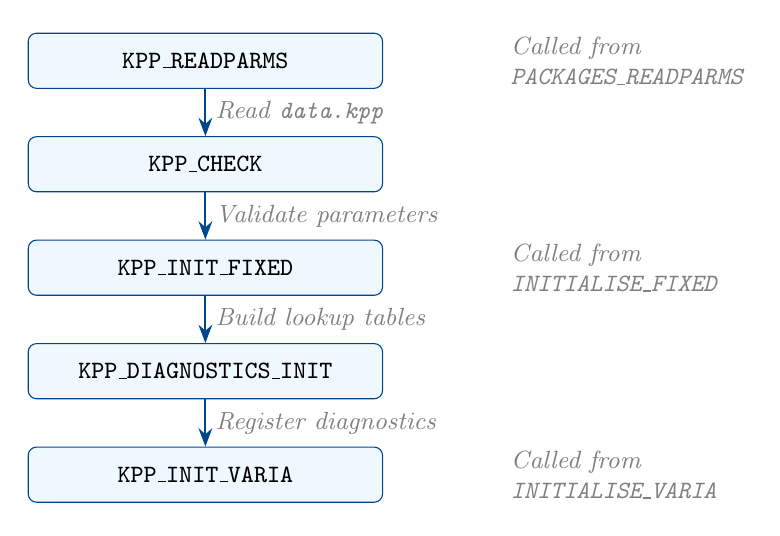
\begin{tikzpicture}[  
  node distance=0.6cm and 2cm,  
  box/.style={rectangle, draw=fortranblue, fill=boxbg,  
              rounded corners=3pt, minimum width=4.5cm,  
              minimum height=0.7cm, font=\small\ttfamily,  
              align=center},  
  arrow/.style={-Stealth, thick, color=fortranblue},  
  label/.style={font=\small\itshape, color=gray}  
]  
  
\node[box] (rp)  {KPP\_READPARMS};  
\node[box, below=of rp] (ch)  {KPP\_CHECK};  
\node[box, below=of ch] (if)  {KPP\_INIT\_FIXED};  
\node[box, below=of if] (di)  {KPP\_DIAGNOSTICS\_INIT};  
\node[box, below=of di] (iv)  {KPP\_INIT\_VARIA};  
  
\draw[arrow] (rp) -- node[right, label]{Read \texttt{data.kpp}} (ch);  
\draw[arrow] (ch) -- node[right, label]{Validate parameters} (if);  
\draw[arrow] (if) -- node[right, label]{Build lookup tables} (di);  
\draw[arrow] (di) -- node[right, label]{Register diagnostics} (iv);  
  
\node[right=1.5cm of rp, label, align=left]  
  {\textit{Called from}\\  
   \texttt{PACKAGES\_READPARMS}};  
\node[right=1.5cm of if, label, align=left]  
  {\textit{Called from}\\  
   \texttt{INITIALISE\_FIXED}};  
\node[right=1.5cm of iv, label, align=left]  
  {\textit{Called from}\\  
   \texttt{INITIALISE\_VARIA}};  
  
\end{tikzpicture}  
\caption{KPP initialization call sequence.}  
\end{figure}  
  
\subsection{Per-Timestep Execution Flow}  
  
The central driver routine \texttt{KPP\_CALC} is called once per tile  
$(bi, bj)$ at a frequency controlled by \texttt{kpp\_freq}. The  
downstream interface routines are called at every model timestep.  
  
\begin{figure}[H]  
\centering  
\begin{tikzpicture}[  
  node distance=0.55cm and 3cm,  
  main/.style={rectangle, draw=fortranblue, fill=boxbg,  
               rounded corners=3pt, minimum width=5.5cm,  
               minimum height=0.65cm, font=\small\ttfamily,  
               align=center, thick},  
  sub/.style={rectangle, draw=fortrangreen!80, fill=fortrangreen!8,  
              rounded corners=2pt, minimum width=4.8cm,  
              minimum height=0.6cm, font=\footnotesize\ttfamily,  
              align=center},  
  out/.style={rectangle, draw=fortranorange, fill=orange!8,  
              rounded corners=2pt, minimum width=4.8cm,  
              minimum height=0.6cm, font=\footnotesize\ttfamily,  
              align=center},  
  arrow/.style={-Stealth, thick, color=fortranblue},  
  sarrow/.style={-Stealth, color=fortrangreen!80},  
  oarrow/.style={-Stealth, color=fortranorange},  
  label/.style={font=\scriptsize\itshape, color=gray, align=left}  
]  
  
% Main chain  
\node[main] (kc)  {KPP\_CALC};  
\node[sub, below=of kc] (sk)  {STATEKPP};  
\node[sub, below=of sk] (ks)  {KPP\_FORCING\_SURF};  
\node[sub, below=of ks] (km)  {KPPMIX};  
  
% KPPMIX children  
\node[sub, right=2.8cm of km] (ri) {Ri\_iwmix};  
\node[sub, above=0.5cm of ri] (z1) {z121};  
\node[sub, below=0.5cm of ri] (bl) {bldepth};  
\node[sub, below=0.5cm of bl] (ws) {wscale};  
\node[sub, below=0.5cm of ws] (bm) {blmix};  
\node[sub, below=0.5cm of bm] (en) {enhance};  
  
% Output routines  
\node[sub, below=0.4cm of km] (tr) {Transfer to KPP* arrays};  
\node[out, below=1.8cm of tr] (cv) {KPP\_CALC\_VISC};  
\node[out, right=0.5cm of cv] (ct) {KPP\_CALC\_DIFF\_T};  
\node[out, below=0.5cm of cv] (cs) {KPP\_CALC\_DIFF\_S};  
\node[out, right=0.5cm of cs] (cp) {KPP\_CALC\_DIFF\_PTR};  
\node[out, below=0.5cm of cs] (tt) {KPP\_TRANSPORT\_T};  
\node[out, right=0.5cm of tt] (ts) {KPP\_TRANSPORT\_S};  
  
% Arrows main chain  
\draw[arrow] (kc) -- (sk);  
\draw[arrow] (sk) -- (ks);  
\draw[arrow] (ks) -- (km);  
\draw[arrow] (km) -- (tr);  
  
% Arrows KPPMIX  
\draw[sarrow] (km.east) -- ++(0.4,0) |- (ri);  
\draw[sarrow] (ri) -- (z1);  
\draw[sarrow] (ri) -- (bl);  
\draw[sarrow] (bl) -- (ws);  
\draw[sarrow] (bl) -- (bm);  
\draw[sarrow] (bm) -- (en);  
  
% Arrows output  
\draw[oarrow] (tr.south) ++(0,0) -- ++(0,-0.35) -| (cv);  
\draw[oarrow] (tr.south) ++(0,0) -- ++(0,-0.35) -| (ct);  
\draw[oarrow] (tr.south) ++(0,0) -- ++(0,-0.35) -| (cs);  
\draw[oarrow] (tr.south) ++(0,0) -- ++(0,-0.35) -| (cp);  
\draw[oarrow] (tr.south) ++(0,0) -- ++(0,-0.35) -| (tt);  
\draw[oarrow] (tr.south) ++(0,0) -- ++(0,-0.35) -| (ts);  
  
\end{tikzpicture}  
\caption{Per-timestep KPP call hierarchy.  
  \textcolor{fortranblue}{Blue}: driver.  
  \textcolor{fortrangreen!80}{Green}: physics subroutines (called within \texttt{KPP\_CALC}).  
  \textcolor{fortranorange}{Orange}: interface routines (called every timestep from  
  main model).}  
\end{figure}  
  
\subsection{Execution Frequency}  
  
A key efficiency feature is that the full KPP calculation is only  
recomputed when required. In \texttt{kpp\_calc.F}, the computation is  
gated by a time-comparison check:  
  
\begin{lstlisting}[  
  language=Fortran90KPP,  
  caption={\texttt{kpp\_calc.F} -- Conditional recomputation of KPP fields.},  
  label={lst:kpp_freq}  
]  
c     Check to see if new vertical mixing coefficient should  
c     be computed now?  
      IF ( DIFFERENT_MULTIPLE(kpp_freq,myTime,deltaTClock)  
     1     .OR. myTime .EQ. startTime ) THEN  
          ...  
          CALL KPPMIX ( ... )  
          ...  
      ENDIF  
\end{lstlisting}  
  
\begin{infobox}  
\textbf{Design implication:} Setting \texttt{kpp\_freq} $>$ \texttt{deltaTClock}  
in \texttt{data.kpp} allows KPP to be computed less frequently than the  
dynamical timestep, e.g.\ once per hour, to reduce cost. The KPP arrays  
(\texttt{KPPviscAz}, \texttt{KPPdiffKzT}, etc.)\ are held constant  
between recomputations.  
\end{infobox}  
  
% ============================================================  
\section{Parameter Initialization}  
% ============================================================  
  
\subsection{\texttt{KPP\_READPARMS} -- Reading \texttt{data.kpp}}  
  
All tunable KPP parameters are read from the Fortran namelist  
\texttt{KPP\_PARM01} within \texttt{data.kpp}. The complete set of  
parameters, their defaults, and their physical meaning is given in  
Table~\ref{tab:params}.  
  
\begin{longtable}{lll p{4.5cm}}  
\toprule  
\textbf{Parameter} & \textbf{Default} & \textbf{Units} &  
\textbf{Description} \\  
\midrule  
\endhead  
\multicolumn{4}{l}{\textit{--- Control ---}} \\  
\texttt{kpp\_freq}      & \texttt{deltaTClock} & s & Recomputation frequency \\  
\texttt{kpp\_dumpFreq}  & \texttt{dumpFreq}    & s & Output dump frequency \\  
\texttt{KPPwriteState}  & \texttt{.FALSE.}     & -- & Write KPP state to file \\  
\texttt{minKPPhbl}      & \texttt{UNSET\_RL}   & m  & Minimum allowed $\hbl$ (no limit if unset) \\  
\midrule  
\multicolumn{4}{l}{\textit{--- Physical constants ---}} \\  
\texttt{epsln}   & $10^{-20}$ & -- & Machine epsilon \\  
\texttt{phepsi}  & $10^{-10}$ & -- & Physical epsilon (division guard) \\  
\texttt{epsilon} & $0.1$      & -- & Nondimensional surface layer fraction \\  
\texttt{vonk}    & $0.4$      & -- & Von K\'{a}rm\'{a}n constant \\  
\texttt{dB\_dz}  & $5.2\times10^{-5}$ & s$^{-2}$ & Max $N^2$ in mixed layer \\  
\midrule  
\multicolumn{4}{l}{\textit{--- Boundary layer depth (bldepth) ---}} \\  
\texttt{Ricr}   & 0.3  & -- & Critical bulk Richardson number \\  
\texttt{cekman} & 0.7  & -- & Ekman depth coefficient \\  
\texttt{cmonob} & 1.0  & -- & Monin-Obukhov depth coefficient \\  
\texttt{concv}  & 1.8  & -- & Interior buoyancy frequency ratio \\  
\texttt{hbf}    & 1.0  & -- & Solar radiation depth fraction \\  
\midrule  
\multicolumn{4}{l}{\textit{--- Interior mixing (Ri\_iwmix) ---}} \\  
\texttt{Riinfty}  & 0.7                  & --     & Shear instability Ri limit \\  
\texttt{BVSQcon}  & $-2\times10^{-5}$   & s$^{-2}$ & Convection N$^2$ threshold \\  
\texttt{difm0}    & $5\times10^{-3}$    & m$^2$/s & Max shear-instability viscosity \\  
\texttt{difs0}    & $5\times10^{-3}$    & m$^2$/s & Max shear-instability scalar diffusivity \\  
\texttt{dift0}    & $5\times10^{-3}$    & m$^2$/s & Max shear-instability heat diffusivity \\  
\texttt{difmcon}  & $0.1$               & m$^2$/s & Convective viscosity \\  
\texttt{difscon}  & $0.1$               & m$^2$/s & Convective scalar diffusivity \\  
\texttt{diftcon}  & $0.1$               & m$^2$/s & Convective heat diffusivity \\  
\midrule  
\multicolumn{4}{l}{\textit{--- Double diffusion (KPP\_DOUBLEDIFF) ---}} \\  
\texttt{Rrho0}   & 1.9                  & -- & Density ratio limit \\  
\texttt{dsfmax}  & $10^{-3}$           & m$^2$/s & Max salt-fingering diffusivity \\  
\midrule  
\multicolumn{4}{l}{\textit{--- Boundary layer mixing (blmix) ---}} \\  
\texttt{cstar}  & 10.0 & -- & Non-local transport proportionality coeff. \\  
\bottomrule  
\caption{KPP run-time parameters read from \texttt{data.kpp}.}  
\label{tab:params}  
\end{longtable}  
  
\subsection{\texttt{KPP\_INIT\_FIXED} -- Time-Invariant Initialization}  
  
This subroutine performs two critical one-time tasks:  
  
\subsubsection{Construction of Turbulent Velocity Scale Lookup Tables}  
  
Because the turbulent velocity scale functions $\wm(\sigma)$ and  
$\ws(\sigma)$ are computed very frequently (inside the inner loops of  
\texttt{bldepth} and \texttt{blmix}), they are pre-tabulated as  
functions of the stability parameter $\hat{\zeta} = \kappa \sigma  
\hbl B_f$ and the friction velocity $\ustar$.  
  
The lookup table dimensions are defined with \texttt{nni}=890 and \texttt{nnj}=480,
giving arrays $[0:\texttt{nni}+1, 0:\texttt{nnj}+1] = [0:891, 0:481]$
with total size $[892, 482]$, spanning:  
\begin{align}  
\hat{\zeta} &\in [\texttt{zmin}, \texttt{zmax}] = [-4\times10^{-7},\ 0]  
\quad \text{m}^3\text{/s}^3 \\  
\ustar &\in [\texttt{umin}, \texttt{umax}] = [0,\ 4\times10^{-2}]  
\quad \text{m/s}  
\end{align}  
  
The table entries follow different formulas for stable/unstable regimes:  
  
\begin{lstlisting}[  
  language=Fortran90KPP,  
  caption={\texttt{kpp\_init\_fixed.F}, lines 135--156 -- Construction of
           \texttt{wmt}/\texttt{wst} lookup tables.},  
  label={lst:lookup}  
]  
      DO i = 0, nni + 1  
         zehat = deltaz*i + zmin  
         DO j = 0, nnj + 1  
            usta = deltau*j + umin  
            zeta = zehat / max(phepsi,usta**3)  
            IF (zehat .GE. 0.) THEN  
c              Stable: both wm and ws follow Monin-Obukhov  
               wmt(i,j) = vonk*usta/(1. + conc1*zeta)  
               wst(i,j) = wmt(i,j)  
            ELSE  
               IF (zeta .GT. zetam) THEN  
c                 Unstable, intermediate regime for momentum  
                  wmt(i,j) = vonk*usta*(1. - conc2*zeta)**p25  
               ELSE  
c                 Unstable, deep convective regime for momentum  
                  wmt(i,j) = vonk*(conam*usta**3 - concm*zehat)**p33  
               ENDIF  
               IF (zeta .GT. zetas) THEN  
c                 Unstable, intermediate regime for scalars  
                  wst(i,j) = vonk*usta*SQRT(1. _d 0 - conc3*zeta)  
               ELSE  
c                 Unstable, deep convective regime for scalars  
                  wst(i,j) = vonk*(conas*usta**3 - concs*zehat)**p33  
               ENDIF  
            ENDIF  
         ENDDO  
      ENDDO  
\end{lstlisting}  
  
The mathematical forms are, for the \textit{unstable} case  
($\hat{\zeta} \leq 0$):  
\begin{align}  
w_m(\sigma) &=  
\begin{cases}  
\kappa \ustar (1 - c_2 \zeta)^{1/4}  
  & \zeta_m < \zeta \leq 0 \\[4pt]  
\kappa (c_{am} \ustar^3 - c_m \hat{\zeta})^{1/3}  
  & \zeta \leq \zeta_m  
\end{cases} \\[6pt]  
w_s(\sigma) &=  
\begin{cases}  
\kappa \ustar \sqrt{1 - c_3 \zeta}  
  & \zeta_s < \zeta \leq 0 \\[4pt]  
\kappa (c_{as} \ustar^3 - c_s \hat{\zeta})^{1/3}  
  & \zeta \leq \zeta_s  
\end{cases}  
\end{align}  
  
where $\zeta = \hat{\zeta}/\ustar^3$ is the stability parameter.  
  
For the \textit{stable} case ($\hat{\zeta} > 0$):  
\begin{equation}  
w_m = w_s = \frac{\kappa \ustar}{1 + c_1 \zeta}  
\end{equation}  
  
\subsubsection{Vertical Grid Setup}  
  
The vertical grid arrays used internally by KPP (\texttt{zgrid},  
\texttt{hwide}) are mapped from the MITgcm model grid:  
  
\begin{lstlisting}[  
  language=Fortran90KPP,  
  caption={\texttt{kpp\_init\_fixed.F}, lines 115--128 -- Mapping  
           of KPP internal grid from MITgcm grid.},  
  label={lst:grid}  
]  
      DO k = 1, Nr  
         zgrid(k) = rC(k)    ! Cell center depth (<=0)  
         hwide(k) = drF(k)   ! Layer thickness (>0)  
      ENDDO  
      zgrid(Nrp1) = zgrid(Nr) * 100.  ! fictitious bottom layer  
      hwide(Nrp1) = phepsi             ! near-zero width  
\end{lstlisting}  
  
\begin{warnbox}  
\textbf{Note:} The fictitious layer at index \texttt{Nrp1} is required  
for the \texttt{blmix} routine, which needs to evaluate diffusivities  
one level below the deepest wet cell. It is assigned a near-zero width  
(\texttt{phepsi}) to avoid unphysical behavior.  
\end{warnbox}  
  
\subsection{\texttt{KPP\_INIT\_VARIA} -- Variable Initialization}  
  
Initializes all time-varying KPP arrays for each tile. Also computes  
\texttt{nzmax(i,j,bi,bj)}, the deepest wet level index (bottom depth  
in model levels), by mapping from \texttt{kLowC}:  
  
\begin{lstlisting}[  
  language=Fortran90KPP,  
  caption={\texttt{kpp\_init\_varia.F}, lines 43--68 -- Array  
           initialization and nzmax computation.},  
  label={lst:initvaria}  
]  
      DO j = 1-OLy, sNy+OLy  
        DO i = 1-OLx, sNx+OLx  
           nzmax(i,j,bi,bj) = kLowC(I,J,bi,bj)  
        ENDDO  
      ENDDO  
      DO k = 1, Nr  
        DO j = 1-OLy, sNy+OLy  
          DO i = 1-OLx, sNx+OLx  
            KPPghat   (i,j,k,bi,bj) = 0.  
            KPPviscAz (i,j,k,bi,bj) = viscArNr(1)  
            KPPdiffKzS(i,j,k,bi,bj) = 0.  
            KPPdiffKzT(i,j,k,bi,bj) = 0.  
          ENDDO  
        ENDDO  
      ENDDO  
\end{lstlisting}  
  
Note that \texttt{KPPviscAz} is initialized to \texttt{viscArNr(1)},  
the background vertical viscosity, rather than zero. This ensures a  
physically reasonable value is present before the first KPP computation.  
  
% ============================================================  
\section{Main Driver: \texttt{KPP\_CALC}}  
% ============================================================  
  
\texttt{KPP\_CALC} (\texttt{kpp\_calc.F}) is the top-level interface  
between the MITgcm ocean model and the KPP mixing routines. It:  
  
\begin{enumerate}[leftmargin=*, label=\textbf{\arabic*.}]  
  \item Checks whether a KPP recomputation is due  
  \item Calls \texttt{STATEKPP} to compute buoyancy-related diagnostics  
  \item Optionally smooths density-derived quantities horizontally  
  \item Constructs surface forcing arrays via \texttt{KPP\_FORCING\_SURF}  
  \item Computes local velocity shear squared (\texttt{shsq})  
  \item Pre-computes background diffusivities via \texttt{CALC\_3D\_DIFFUSIVITY}  
  \item Optionally adds double diffusion via \texttt{KPP\_DOUBLEDIFF}  
  \item Calls \texttt{KPPMIX} to compute boundary layer mixing  
  \item Transfers results to global arrays with land masking  
  \item Computes shortwave and salt-plume fraction fields  
\end{enumerate}  
  
\subsection{Velocity Shear Computation}  
  
Two shear-squared quantities are computed within \texttt{KPP\_CALC}:  
  
\paragraph{Local shear \texttt{shsq}} (for Richardson number in the interior):  
\begin{equation}  
\texttt{shsq}_{k} = \frac{1}{2}\left[  
  (u_k - u_{k+1})^2 + (u_{k+1, \text{east}} - u_{k+1+1, \text{east}})^2 +  
  (v_k - v_{k+1})^2 + (v_{k, \text{north}} - v_{k+1, \text{north}})^2  
\right]  
\end{equation}  
This averages the velocity shear from the u,v-grid onto the t-grid.  
  
When \texttt{KPP\_SMOOTH\_SHSQ} is defined (default), a 121 horizontal  
filter is applied using contributions from neighboring columns:  
  
\begin{lstlisting}[  
  language=Fortran90KPP,  
  caption={\texttt{kpp\_calc.F}, lines $\sim$185--210 -- Horizontal  
           smoothing of \texttt{shsq} with 121 filter.},  
  label={lst:shsq_smooth}  
]  
#ifdef KPP_SMOOTH_SHSQ  
         shsq(i,j,k) = p5 * shsq(i,j,k) + p125 * (  
     &        (uVel(i,  jm1,k,bi,bj)-uVel(i,  jm1,kp1,bi,bj)) *  
     &        (uVel(i,  jm1,k,bi,bj)-uVel(i,  jm1,kp1,bi,bj)) +  
     &        ... [8 more neighbor contributions] ...  
     &        (vVel(ip1,jp1,k,bi,bj)-vVel(ip1,jp1,kp1,bi,bj)) *  
     &        (vVel(ip1,jp1,k,bi,bj)-vVel(ip1,jp1,kp1,bi,bj)) )  
#endif  
\end{lstlisting}  
  
The smoothing weights are: center $= 0.5$, face neighbors $= 0.125$  
each (total $= 4 \times 0.125 = 0.5$), summing to 1.  
  
\paragraph{Surface-referenced shear \texttt{dVsq}} (for bulk Richardson  
number in boundary layer depth search):  
\begin{equation}  
\texttt{dVsq}_{k} = \frac{1}{2}\left[  
  (U_{\rm ref} - u_k)^2 + \ldots + (V_{\rm ref} - v_{k,\rm north})^2  
\right]  
\end{equation}  
where $U_{\rm ref}$, $V_{\rm ref}$ are the surface layer velocities  
(or an estimated reference velocity if \texttt{KPP\_ESTIMATE\_UREF} is  
defined).  
  
\subsection{Background Diffusivity and Double Diffusion}  
  
Before calling \texttt{KPPMIX}, background diffusivities are computed  
by calling the standard MITgcm routine \texttt{CALC\_3D\_DIFFUSIVITY}:  
  
\begin{lstlisting}[  
  language=Fortran90KPP,  
  caption={\texttt{kpp\_calc.F} -- Background diffusivity computation  
           and optional double-diffusion enhancement.},  
  label={lst:background}  
]  
      CALL CALC_3D_DIFFUSIVITY(  
     I        bi,bj,1-OLx,sNx+OLx,1-OLy,sNy+OLy,  
     I        GAD_SALINITY, .FALSE., .FALSE.,  
     O        KPPdiffKzS(1-OLx,1-OLy,1,bi,bj),  
     I        myThid)  
      CALL CALC_3D_DIFFUSIVITY(  
     I        bi,bj,1-OLx,sNx+OLx,1-OLy,sNy+OLy,  
     I        GAD_TEMPERATURE, .FALSE., .FALSE.,  
     O        KPPdiffKzT(1-OLx,1-OLy,1,bi,bj),  
     I        myThid)  
#ifndef EXCLUDE_KPP_DOUBLEDIFF  
      IF ( KPPuseDoubleDiff ) THEN  
       CALL KPP_DOUBLEDIFF(  
     I      TTALPHA, SSBETA,  
     U      KPPdiffKzT(1-OLx,1-OLy,1,bi,bj),  
     U      KPPdiffKzS(1-OLx,1-OLy,1,bi,bj),  
     I      ikey,1-OLx,sNx+OLx,1-OLy,sNy+OLy,bi,bj,myThid)  
      ENDIF  
#endif  
\end{lstlisting}  
  
These background diffusivities serve two roles: (1) they provide the  
interior diffusivity baseline upon which shear instability and convective  
mixing add incremental contributions in \texttt{Ri\_iwmix}, and (2) they  
allow the KPP boundary layer diffusivity to match the interior value  
at $z = -\hbl$ (the matching/smoothing condition in \texttt{blmix}).  
  
\subsection{Result Transfer and Masking}  
  
After \texttt{KPPMIX} returns, the 1-D internal arrays \texttt{vddiff}  
(indexed as \texttt{(x,y,0:Nrp1,mdiff)}) are transferred to the 3-D  
global arrays with land masking applied:  
  
\begin{lstlisting}[  
  language=Fortran90KPP,  
  caption={\texttt{kpp\_calc.F} -- Transfer of \texttt{KPPMIX} output  
           to global KPP arrays with masking.},  
  label={lst:transfer}  
]  
      DO k = 1, Nr  
       km1 = max(1,k-1)  
       DO j = jMin, jMax  
        DO i = iMin, iMax  
         KPPviscAz(i,j,k,bi,bj) = vddiff(i,j,k-1,1)  
     &        * maskC(i,j,k,bi,bj) * maskC(i,j,km1,bi,bj)  
         KPPdiffKzS(i,j,k,bi,bj)= vddiff(i,j,k-1,2)  
     &        * maskC(i,j,k,bi,bj) * maskC(i,j,km1,bi,bj)  
         KPPdiffKzT(i,j,k,bi,bj)= vddiff(i,j,k-1,3)  
     &        * maskC(i,j,k,bi,bj) * maskC(i,j,km1,bi,bj)  
         KPPghat(i,j,k,bi,bj)   = ghat(i,j,k)  
     &        * maskC(i,j,k,bi,bj) * maskC(i,j,km1,bi,bj)  
        ENDDO  
       ENDDO  
      ENDDO  
\end{lstlisting}  
  
The double masking (\texttt{maskC(k)} $\times$ \texttt{maskC(km1)})  
ensures that diffusivities are zero at interfaces adjacent to land  
or seafloor cells.  
  
% ============================================================  
\section{Density and Buoyancy: \texttt{STATEKPP}}  
% ============================================================  
  
Located in \texttt{kpp\_routines.F}, \texttt{STATEKPP} computes all  
density-related input fields needed by the KPP scheme. It calls the  
standard MITgcm equation-of-state routines \texttt{FIND\_RHO\_2D},  
\texttt{FIND\_ALPHA}, and \texttt{FIND\_BETA}.  
  
\subsection{Outputs}  
  
\begin{longtable}{lp{8cm}l}  
\toprule  
\textbf{Variable} & \textbf{Definition} & \textbf{Units} \\  
\midrule  
\endhead  
\texttt{RHO1} & Surface layer potential density:  
  $\rho_1 = \rho(T_1, S_1, p_1) + \rho_0$ & kg/m$^3$ \\[4pt]  
\texttt{TTALPHA} & Thermal expansion:  
  $\alpha = \partial\rho/\partial T$ & kg/m$^3$/°C \\[4pt]  
\texttt{SSBETA} & Haline contraction:  
  $\beta = \partial\rho/\partial S$ & kg/m$^3$/(g/kg) \\[4pt]  
\texttt{DBLOC}$(k)$ & Local buoyancy gradient across interface $k$:  
  $\delta b_{\rm loc}(k) = g(\rho_k - \rho_{k-1})/\rho_k$ & m/s$^2$ \\[4pt]  
\texttt{DBSFC}$(k)$ & Buoyancy difference w.r.t.\ surface:  
  $\delta b_{\rm sfc}(k) = g(\rho_k - \rho_{1k})/\rho_k$ & m/s$^2$ \\  
\bottomrule  
\end{longtable}  
  
\subsection{Key Density Calls}  
  
For each level $k \geq 2$, three density evaluations are made:  
  
\begin{lstlisting}[  
  language=Fortran90KPP,  
  caption={\texttt{kpp\_routines.F} (\texttt{STATEKPP}) -- Density  
           evaluations for buoyancy gradient computation.},  
  label={lst:statekpp}  
]  
c     RHOK   = rho( T(k),   S(k),   pressure(k) )  
         CALL FIND_RHO_2D( ..., k, theta(:,:,k,:,:),  
     O        RHOK, k, bi, bj, myThid )  
  
c     RHOKM1 = rho( T(k-1), S(k-1), pressure(k) ) -- at level k!  
c     This evaluates the density of the overlying layer at the  
c     pressure of the current layer (adiabatic displacement)  
         CALL FIND_RHO_2D( ..., k, theta(:,:,k-1,:,:),  
     O        RHOKM1, k-1, bi, bj, myThid )  
  
c     RHO1K  = rho( T(1),   S(1),   pressure(k) ) -- surface parcel  
c     displaced adiabatically to level k (for bulk Richardson number)  
         CALL FIND_RHO_2D( ..., k, theta(:,:,1,:,:),  
     O        RHO1K, 1, bi, bj, myThid )  
\end{lstlisting}  
  
This gives the physically correct definition of static stability  
(accounting for adiabatic compressibility) and bulk density difference:  
  
\begin{align}  
\delta b_{\rm loc}(k-1) &= g\,\frac{\rho_k - \rho_{k-1}}{\rho_k + \rho_0}  
\quad \text{(local buoyancy gradient)} \\[6pt]  
\delta b_{\rm sfc}(k) &= g\,\frac{\rho_k - \rho_{1k}}{\rho_k + \rho_0}  
\quad \text{(surface-referenced buoyancy deficit)}  
\end{align}  
  
Note that \texttt{DBLOC(k)} is defined at the \textit{bottom} of cell $k$  
(i.e., at the interface between cells $k$ and $k+1$ in MITgcm indexing),  
not at the top. This has important implications for masking: the correct  
mask is \texttt{maskC(k)} $\times$ \texttt{maskC(k+1)}.  
  
% ============================================================  
\section{Surface Forcing: \texttt{KPP\_FORCING\_SURF}}  
% ============================================================  
  
Located in \texttt{kpp\_forcing\_surf.F}, this subroutine converts  
model surface forcing fields (in MITgcm units) into the three  
surface forcing quantities required by KPP.  
  
\subsection{Friction Velocity}  
  
The surface friction velocity $\ustar$ is derived from the wind stress:  
  
\begin{equation}  
\ustar = \sqrt{\sqrt{\tau_x^2 + \tau_y^2} / \rho_{\rm surf}}  
\end{equation}  
  
where $\tau_x$, $\tau_y$ are the zonal and meridional wind stresses  
(\texttt{surfaceForcingU}, \texttt{surfaceForcingV} in MITgcm).  
The implementation averages the u,v-grid stresses onto the t-grid:  
  
\begin{lstlisting}[  
  language=Fortran90KPP,  
  caption={\texttt{kpp\_forcing\_surf.F}, lines $\sim$130--155 --  
           Computation of friction velocity \texttt{ustar}.},  
  label={lst:ustar}  
]  
      DO j = jmin, jmax  
       jp1 = j + 1  
       DO i = imin, imax  
        ip1 = i+1  
        work3(i,j) =  
     &   (surfForcU(i,j,bi,bj) + surfForcU(ip1,j,bi,bj)) *  
     &   (surfForcU(i,j,bi,bj) + surfForcU(ip1,j,bi,bj)) +  
     &   (surfForcV(i,j,bi,bj) + surfForcV(i,jp1,bi,bj)) *  
     &   (surfForcV(i,j,bi,bj) + surfForcV(i,jp1,bi,bj))  
       ENDDO  
      ENDDO  
      epsLocSq = phepsi*phepsi*drF(1)*drF(1)  
      epsLoc   = SQRT ( p5*phepsi*drF(1) )  
      DO j = jmin, jmax  
       DO i = imin, imax  
        IF ( work3(i,j) .lt. epsLocSq ) THEN  
           ustar(i,j) = epsLoc  
        ELSE  
           tempVar2 =  SQRT( work3(i,j) ) * p5  
           ustar(i,j) = SQRT( tempVar2 )  
        ENDIF  
       ENDDO  
      ENDDO  
\end{lstlisting}  
  
\subsection{Surface Buoyancy Fluxes}  
  
\paragraph{Turbulent buoyancy flux \texttt{bo}:}  
\begin{equation}  
B_0 = -\frac{g}{\rho_{\rm surf}}\left[\alpha\,(Q_T + Q_{\rm ice})  
+ \beta\,(E - P - R)\cdot S_{\rm surf}\right]  
\end{equation}  
  
\begin{lstlisting}[  
  language=Fortran90KPP,  
  caption={\texttt{kpp\_forcing\_surf.F} -- Turbulent surface  
           buoyancy forcing.},  
  label={lst:bo}  
]  
      DO j = jmin, jmax  
       DO i = imin, imax  
        bo(i,j) = - gravity *  
     &       ( TTALPHA(i,j,1) * (surfForcT(i,j,bi,bj)+  
     &       surfForcTice(i,j,bi,bj)) +  
     &       SSBETA(i,j,1) * surfForcS(i,j,bi,bj) )  
     &       / rhoSurf(i,j)  
       ENDDO  
      ENDDO  
\end{lstlisting}  
  
\paragraph{Radiative (shortwave) buoyancy flux \texttt{bosol}:}  
\begin{equation}  
B_{0,\rm sol} = \frac{g\,\alpha\,Q_{\rm sw}}{C_p\,\rho_0\,\rho_{\rm surf}}  
\end{equation}  
  
This is the component of surface buoyancy forcing due to shortwave  
radiation. It is separated from \texttt{bo} because it penetrates  
below the surface and its contribution to the mixed layer heat budget  
depends on the depth profile of absorption.  
  
\paragraph{Haline buoyancy flux from salt plumes \texttt{boplume}:}  
When \texttt{ALLOW\_SALT\_PLUME} is defined:  
\begin{equation}  
B_{\rm plume} = -\frac{g\,\beta\,F_{\rm SP}}{\rho_0^2}  
\end{equation}  
where $F_{\rm SP}$ is the downward salt flux from brine rejection.  
  
\subsection{Surface-Referenced Velocity Shear \texttt{dVsq}}  
  
Without \texttt{KPP\_ESTIMATE\_UREF}, the shear is referenced to the  
top model level:  
\begin{equation}  
\texttt{dVsq}(k) = \frac{1}{2}\sum_{\rm neighbors}  
\left[(U_1 - U_k)^2 + (V_1 - V_k)^2\right]  
\end{equation}  
  
% ============================================================  
\section{Core Solver: \texttt{KPPMIX}}  
% ============================================================  
  
\texttt{KPPMIX} is the master driver for the one-dimensional KPP column  
calculations. It calls the four core physics routines in sequence and  
combines their outputs.  
  
The data flow through \texttt{KPPMIX} is:  
  
\begin{enumerate}[leftmargin=*, label=\textbf{\arabic*.}]  
  \item \texttt{Ri\_iwmix} $\rightarrow$ interior mixing coefficients  
        in \texttt{diffus(:,:,1:3)}  
  \item Set seafloor and sub-bottom values to zero in \texttt{diffus}  
  \item \texttt{bldepth} $\rightarrow$ boundary layer depth \texttt{hbl},  
        stability flags, bulk Richardson numbers  
  \item \texttt{blmix} $\rightarrow$ boundary layer mixing \texttt{blmc}  
        and non-local term \texttt{ghat}  
  \item \texttt{enhance} $\rightarrow$ smooth diffusivity at $z = -\hbl$  
  \item Combine: use \texttt{blmc} above \texttt{kbl}, \texttt{diffus}  
        below; zero \texttt{ghat} below \texttt{kbl}  
\end{enumerate}  
  
\begin{lstlisting}[  
  language=Fortran90KPP,  
  caption={\texttt{kpp\_routines.F} (\texttt{KPPMIX}) -- Final combination  
           of interior and boundary layer diffusivities.},  
  label={lst:kppmix_combine}  
]  
      DO k = 1, Nr  
       DO i = 1, imt  
        IF (k .LT. kbl(i)) THEN  
c          Within boundary layer: use blmix result  
           diffus(i,k,1) = MAX ( blmc(i,k,1), viscArNr(1) )  
           diffus(i,k,2) = MAX ( blmc(i,k,2), diffusKzS(i,Nr) )  
           diffus(i,k,3) = MAX ( blmc(i,k,3), diffusKzT(i,Nr) )  
        ELSE  
c          Below boundary layer: ghat is zero  
           ghat(i,k) = 0. _d 0  
        ENDIF  
       ENDDO  
      ENDDO  
\end{lstlisting}  
  
Note the use of \texttt{MAX}: this ensures the boundary layer  
diffusivity is never less than the background viscosity  
(\texttt{viscArNr(1)}) or the deep interior diffusivity. This is a  
numerical safeguard for shallow mixed layers.  
  
% ============================================================  
\section{Interior Mixing: \texttt{Ri\_iwmix}}  
% ============================================================  
  
\texttt{Ri\_iwmix} computes vertical diffusivities at all interfaces  
$k = 1, \ldots, N_r$ due to three mechanisms: (1) background internal  
wave activity, (2) shear instability, and (3) static instability  
(convection).  
  
\subsection{Richardson Number Computation}  
  
The local gradient Richardson number is computed from the smoothed  
buoyancy gradient and the local velocity shear:  
  
\begin{equation}  
\Ri_{\rm loc}(k) = \frac{\delta b_{\rm loc,sm}(k) \cdot  
(z_k - z_{k+1})}{\max(\texttt{shsq}(k),\ \varepsilon)}  
\end{equation}  
  
where \texttt{dblocSm} is the horizontally smoothed version of  
\texttt{dbloc} (stored in \texttt{ghat} temporarily to save memory):  
  
\begin{lstlisting}[  
  language=Fortran90KPP,  
  caption={\texttt{kpp\_routines.F} (\texttt{Ri\_iwmix}) -- Local  
           Richardson number computation.},  
  label={lst:riwmix}  
]  
      DO ki = 1, Nr  
         DO i = 1, imt  
            IF     (kmtj(i) .LE. 1      ) THEN  
               diffus(i,ki,1) = 0.  
               diffus(i,ki,2) = 0.  
            ELSEIF (ki      .GE. kmtj(i)) THEN  
c              At/below seafloor: use last valid value  
               diffus(i,ki,1) = diffus(i,ki-1,1)  
               diffus(i,ki,2) = diffus(i,ki-1,2)  
            ELSE  
c              Interior: compute Ri from smoothed dbloc / shsq  
               diffus(i,ki,1) = dblocSm(i,ki) * (zgrid(ki)-zgrid(ki+1))  
     &            / MAX( Shsq(i,ki), phepsi )  
               diffus(i,ki,2) = dbloc(i,ki) / (zgrid(ki)-zgrid(ki+1))  
            ENDIF  
         ENDDO  
      ENDDO  
\end{lstlisting}  
  
Here \texttt{diffus(:,:,1)} temporarily stores the Richardson number,  
and \texttt{diffus(:,:,2)} stores $N^2$ (Brunt-V\"{a}is\"{a}l\"{a}  
frequency squared). These are overwritten with the actual diffusivities  
in the next step.  
  
\subsection{Mixing Functions}  
  
Two nonlinear functions of the Richardson number control the strength  
of mixing:  
  
\paragraph{Convective mixing function $f_{\rm con}$:}  
\begin{equation}  
f_{\rm con} = \left[1 - \left(\min\!\left(\frac{N^2_{\rm con} - N^2}{N^2_{\rm con}},\  
1\right)\right)^2\right]^3  
\end{equation}  
where $N^2_{\rm con} = \texttt{BVSQcon} = -2\times10^{-5}$~s$^{-2}$.  
This is active ($f_{\rm con} > 0$) only when $N^2 < 0$, i.e.\ the  
water column is statically unstable.  
  
\paragraph{Shear instability function $f_\Ri$:}  
\begin{equation}  
f_\Ri = \left[1 - \left(\min\!\left(\frac{\Ri}{\Ri_\infty},\ 1\right)\right)^2\right]^3  
\end{equation}  
where $\Ri_\infty = \texttt{Riinfty} = 0.7$. This goes from 1 (at  
$\Ri = 0$) to 0 (at $\Ri \geq \Ri_\infty$).  
  
\begin{lstlisting}[  
  language=Fortran90KPP,  
  caption={\texttt{kpp\_routines.F} (\texttt{Ri\_iwmix}) -- Evaluation  
           of mixing functions and diffusivities.},  
  label={lst:fcon_fri}  
]  
      DO ki = 1, Nr  
         DO i = 1, imt  
c           f of Brunt-Vaisala squared for convection  
            Rig   = MAX ( diffus(i,ki,2) , BVSQcon )  
            ratio = MIN ( (BVSQcon - Rig) / BVSQcon, c1 )  
            fcon  = c1 - ratio * ratio  
            fcon  = fcon * fcon * fcon  
  
c           f of smooth Ri for shear instability  
            Rig   = MAX ( diffus(i,ki,1), c0 )  
            ratio = MIN ( Rig / Riinfty , c1 )  
            fRi   = c1 - ratio * ratio  
            fRi   = fRi * fRi * fRi  
  
c           Final diffusivities  
            kp1 = MIN(ki+1,Nr)  
            diffus(i,ki,1) = viscArNr(1) + fcon*difmcon + fRi*difm0  
            diffus(i,ki,2) = diffusKzS(i,kp1)+fcon*difscon+fRi*difs0  
            diffus(i,ki,3) = diffusKzT(i,kp1)+fcon*diftcon+fRi*dift0  
         ENDDO  
      ENDDO  
\end{lstlisting}  
  
The resulting interior diffusivities at each interface are:  
\begin{align}  
\kappa_m(k) &= \nu_{\rm bg} + f_{\rm con} \cdot \nu_{\rm con}  
               + f_\Ri \cdot \nu_{\rm shear} \\[4pt]  
\kappa_S(k) &= \kappa_{S,{\rm bg}}(k{+}1) + f_{\rm con} \cdot  
               \kappa_{S,{\rm con}} + f_\Ri \cdot \kappa_{S,{\rm shear}} \\[4pt]  
\kappa_T(k) &= \kappa_{T,{\rm bg}}(k{+}1) + f_{\rm con} \cdot  
               \kappa_{T,{\rm con}} + f_\Ri \cdot \kappa_{T,{\rm shear}}  
\end{align}  
  
\begin{infobox}  
\textbf{Background diffusivity indexing:} The background diffusivities  
(\texttt{diffusKzS(i,kp1)}, \texttt{diffusKzT(i,kp1)}) are taken at  
level $k+1$ (one level below the current interface). This means the  
background at the bottom interface of cell $k$ uses the background  
diffusivity representative of the cell below.  
\end{infobox}  
  
\subsection{Vertical Smoothing of Ri (\texttt{z121})}  
  
When \texttt{ALLOW\_KPP\_VERTICALLY\_SMOOTH} is defined, the Richardson  
number stored in \texttt{diffus(:,:,1)} is smoothed vertically using  
the 121 filter \texttt{z121}. This filter applies the stencil  
$[1/4,\ 1/2,\ 1/4]$ in the vertical, but \textit{only to grid points  
where $0 \leq \Ri \leq \Ri_\infty$} (within the turbulent mixing range).  
This prevents smoothing from contaminating convectively unstable regions  
or quiescent stratified regions.  
  
% ============================================================  
\section{Boundary Layer Depth: \texttt{bldepth}}  
% ============================================================  
  
\texttt{bldepth} determines the depth of the oceanic planetary boundary  
layer $\hbl$ by searching downward for the level at which the bulk  
Richardson number first exceeds the critical value $\Ricr = 0.3$.  
  
\subsection{Bulk Richardson Number}  
  
The bulk Richardson number at level $k$ is:  
\begin{equation}  
\Ri_b(k) = \frac{\texttt{Ritop}(k)}{\texttt{dVsq}(k) + V_t^2(k)}  
= \frac{(z_{\rm ref} - z_k)\,\delta b_{\rm sfc}(k)}  
  {(U_{\rm ref} - U_k)^2 + (V_{\rm ref} - V_k)^2 + V_t^2(k)}  
\end{equation}  
  
where the turbulent shear term $V_t^2$ accounts for the unresolved  
contribution of sub-grid turbulence to the denominator:  
  
\begin{equation}  
V_t^2(k) = -z_k \cdot w_s \cdot \sqrt{|N_k^2|} \cdot V_{tc}  
\end{equation}  
  
\begin{lstlisting}[  
  language=Fortran90KPP,  
  caption={\texttt{kpp\_routines.F} (\texttt{bldepth}) -- Turbulent  
           shear term and bulk Richardson number.},  
  label={lst:Ribulk}  
]  
         DO i = 1, imt  
c           Estimate N^2 at this level from adjacent dbloc values  
            bvsq = p5 *  
     1           ( dbloc(i,kl-1) / (zgrid(kl-1)-zgrid(kl  ))+  
     2             dbloc(i,kl  ) / (zgrid(kl  )-zgrid(kl+1)))  
            IF (bvsq .EQ. 0. _d 0) THEN  
              vtsq = 0. _d 0  
            ELSE  
c             Turbulent shear contribution  
              vtsq = -zgrid(kl) * ws(i) * SQRT(ABS(bvsq)) * Vtc  
            ENDIF  
c           Bulk Richardson number  
            tempVar1  = dvsq(i,kl) + vtsq  
            tempVar2 = MAX(tempVar1, phepsi)  
            Rib(i,kl) = Ritop(i,kl) / tempVar2  
         ENDDO  
\end{lstlisting}  
  
\subsection{Linear Interpolation for \texttt{hbl}}  
  
Once the level $k = k_{\rm bl}$ where $\Ri_b$ first exceeds $\Ricr$ is  
identified, $\hbl$ is obtained by linear interpolation:  
  
\begin{equation}  
\hbl = -z_{k-1} + (z_{k-1} - z_k)\,\frac{\Ricr - \Ri_b(k-1)}  
                                          {\Ri_b(k) - \Ri_b(k-1)}  
\end{equation}  
  
\begin{lstlisting}[  
  language=Fortran90KPP,  
  caption={\texttt{kpp\_routines.F} (\texttt{bldepth}) -- Linear  
           interpolation to find exact \texttt{hbl}.},  
  label={lst:hbl_interp}  
]  
      DO i = 1, imt  
         kl = kbl(i)  
c        linearly interpolate to find hbl where Rib = Ricr  
         IF (kl.GT.1 .AND. kl.LT.kmtj(i)) THEN  
            tempVar1 = (Rib(i,kl)-Rib(i,kl-1))  
            hbl(i) = -zgrid(kl-1) + (zgrid(kl-1)-zgrid(kl)) *  
     1           (Ricr - Rib(i,kl-1)) / tempVar1  
         ENDIF  
      ENDDO  
\end{lstlisting}  
  
\subsection{Stability Limits on \texttt{hbl}}  
  
Under stable surface forcing ($B_f > 0$), \texttt{hbl} is additionally  
limited by Ekman depth and Monin-Obukhov depth:  
  
\begin{align}  
h_{\rm Ekman} &= c_{\rm Ekman}\,\frac{\ustar}{|f|} \\[4pt]  
h_{\rm MO} &= c_{\rm MO}\,\frac{\ustar^3}{\kappa\,B_f} \\[4pt]  
\hbl &= \min\!\left(\hbl,\ \min(h_{\rm Ekman},\ h_{\rm MO})\right)  
\quad \text{(stable conditions only)}  
\end{align}  
  
\begin{lstlisting}[  
  language=Fortran90KPP,  
  caption={\texttt{kpp\_routines.F} (\texttt{bldepth}) -- Ekman and  
           Monin-Obukhov depth limits.},  
  label={lst:hbl_limits}  
]  
      IF ( LimitHblStable ) THEN  
       DO i = 1, imt  
        IF (bfsfc(i) .GT. 0.0) THEN  
         hekman = cekman * ustar(i) / MAX(ABS(Coriol(i)),phepsi)  
         hmonob = cmonob * ustar(i)*ustar(i)*ustar(i)  
     &        / vonk / bfsfc(i)  
         hlimit = stable(i) * MIN(hekman,hmonob)  
     &        + (stable(i)-1.) * zgrid(Nr)  
         hbl(i) = MIN(hbl(i),hlimit)  
        ENDIF  
       ENDDO  
      ENDIF  
\end{lstlisting}  
  
Finally, \texttt{hbl} is constrained from below by \texttt{minKPPhbl}  
(default: depth of first model level center):  
\begin{equation}  
\hbl = \max(\hbl,\ \hbl_{\min})  
\end{equation}  
  
\subsection{Case A / Case B Classification}  
  
After determining \texttt{hbl}, the subroutine classifies each column  
as Case A or Case B, which determines how the matching between boundary  
layer and interior diffusivities is handled in \texttt{blmix}:  
  
\begin{equation}  
\texttt{caseA}(i) = \begin{cases}  
1 & \text{if } -z_{k_{\rm bl}} - \tfrac{1}{2}h_{k_{\rm bl}} > \hbl  
    \quad \text{(hbl is within cell kbl)} \\  
0 & \text{otherwise (hbl is at cell boundary)}  
\end{cases}  
\end{equation}  
  
% ============================================================  
\section{Turbulent Velocity Scales: \texttt{wscale}}  
% ============================================================  
  
Given $\sigma$ (normalized depth), $\hbl$, $\ustar$, and the total  
surface buoyancy flux $\bfsfc$, \texttt{wscale} returns the turbulent  
velocity scales $\wm$ and $\ws$ by bilinear interpolation in the  
pre-computed lookup tables.  
  
\subsection{Bilinear Interpolation}  
  
\begin{lstlisting}[  
  language=Fortran90KPP,  
  caption={\texttt{kpp\_routines.F} (\texttt{wscale}) -- Bilinear  
           interpolation in wm/ws lookup tables.},  
  label={lst:wscale}  
]  
      DO i = 1, imt  
         zehat = vonk*sigma(i)*hbl(i)*bfsfc(i)  
  
         IF (zehat .LE. zmax) THEN  
c           Use lookup table  
            zdiff = zehat - zmin  
            iz    = MIN( MAX(INT( zdiff / deltaz ), 0), nni )  
            izp1  = iz + 1  
            udiff = ustar(i) - umin  
            ju    = MIN( MAX(INT( udiff / deltau ), 0), nnj )  
            jup1  = ju + 1  
  
            zfrac = zdiff / deltaz - float(iz)  
            ufrac = udiff / deltau - float(ju)  
            fzfrac= 1. - zfrac  
  
c           Bilinear interpolation for wm  
            wam   = fzfrac * wmt(iz,jup1) + zfrac * wmt(izp1,jup1)  
            wbm   = fzfrac * wmt(iz,ju  ) + zfrac * wmt(izp1,ju  )  
            wm(i) = (1.-ufrac) * wbm      + ufrac * wam  
         ELSE  
c           Stable conditions outside table range  
            u3 = ustar(i) * ustar(i) * ustar(i)  
            wm(i) = vonk * ustar(i) * u3 / (u3 + conc1 * zehat)  
            ws(i) = wm(i)  
         ENDIF  
      ENDDO  
\end{lstlisting}  
  
% ============================================================  
\section{Boundary Layer Mixing: \texttt{blmix}}  
% ============================================================  
  
\texttt{blmix} computes turbulent diffusivities and viscosities  
\textit{within} the boundary layer using a cubic polynomial profile.  
  
\subsection{Shape Function $G(\sigma)$}  
  
The KPP boundary layer mixing profile has the form:  
\begin{equation}  
K(\sigma) = h_{\rm bl}\,w(\sigma)\,\sigma\,G(\sigma)  
\end{equation}  
  
where the shape function $G(\sigma)$ is a cubic polynomial in $\sigma$:  
\begin{equation}  
G(\sigma) = a_1 + a_2\,g_1 + a_3\,g_1'  
\end{equation}  
  
with $a_1 = \sigma - 2$, $a_2 = 3 - 2\sigma$, $a_3 = \sigma - 1$,  
and the matching conditions at $\sigma = 1$ (i.e.\ at $z = -\hbl$):  
\begin{equation}  
g_1 = K(\hbl)/(h_{\rm bl}\,w(1)),  
\qquad  
g_1' = \frac{dK/d\sigma|_{\sigma=1}}{w(1)} + f_1 K(\hbl)  
\end{equation}  
  
The constant $f_1$ stabilizes the profile under stable forcing:  
\begin{equation}  
f_1 = c_1\,\frac{B_f}{\max(\ustar^4, \varepsilon)}  
\end{equation}  
  
\begin{lstlisting}[  
  language=Fortran90KPP,  
  caption={\texttt{kpp\_routines.F} (\texttt{blmix}) -- Shape function  
           and boundary layer diffusivity computation.},  
  label={lst:blmix_G}  
]  
         DO i = 1, imt  
            sig = (-zgrid(ki) + 0.5 * hwide(ki)) / hbl(i)  
            a1 = sig - 2.  
            a2 = 3. - 2. * sig  
            a3 = sig - 1.  
  
c           Dimensionless shape functions  
            Gm = a1 + a2 * gat1m(i) + a3 * dat1m(i)  
            Gs = a1 + a2 * gat1s(i) + a3 * dat1s(i)  
            Gt = a1 + a2 * gat1t(i) + a3 * dat1t(i)  
  
c           Boundary layer diffusivities  
            blmc(i,ki,1) = hbl(i) * wm(i) * sig * (1. + sig * Gm)  
            blmc(i,ki,2) = hbl(i) * ws(i) * sig * (1. + sig * Gs)  
            blmc(i,ki,3) = hbl(i) * ws(i) * sig * (1. + sig * Gt)  
         ENDDO  
\end{lstlisting}  
  
The matching conditions $g_1$ (\texttt{gat1m/s/t}) and $g_1'$  
(\texttt{dat1m/s/t}) are computed at the top of \texttt{blmix} by  
evaluating the interior diffusivities and their gradients at $z = -\hbl$:  
  
\begin{lstlisting}[  
  language=Fortran90KPP,  
  caption={\texttt{kpp\_routines.F} (\texttt{blmix}) -- Computation of  
           matching conditions at $z = -\hbl$.},  
  label={lst:blmix_match}  
]  
c        Find diffusivities and derivative at hbl  
         delhat = 0.5*hwide(kn) - zgrid(kn) - hbl(i)  
         R      = 1.0 - delhat / hwide(kn)  
c        Gradient of interior viscosity at kn interface  
         dvdzup = (diffus(i,kn-1,1) - diffus(i,kn  ,1)) / hwide(kn)  
         dvdzdn = (diffus(i,kn  ,1) - diffus(i,kn+1,1)) / hwide(kn+1)  
         viscp  = 0.5 * ( (1.-R) * (dvdzup + ABS(dvdzup)) +  
     1                        R  * (dvdzdn + ABS(dvdzdn))  )  
         visch  = diffus(i,kn,1) + viscp * delhat  
  
c        Matching conditions  
         gat1m(i) = visch / hbl(i) / wm(i)  
         dat1m(i) = -viscp / wm(i) + f1 * visch  
\end{lstlisting}  
  
\subsection{Non-local Transport Term}  
  
Under unstable (convective) surface forcing, a counter-gradient  
non-local transport term $\ghat$ is activated:  
  
\begin{equation}  
\ghat(k) = (1 - s_{\rm stable})\,\frac{c_g}  
            {\max(w_s(\sigma_k)\,\hbl,\ \varepsilon)}  
\end{equation}  
  
where $c_g = c^* \kappa (c_s \kappa \epsilon)^{1/3}$ (computed in  
\texttt{KPP\_INIT\_FIXED}) and $s_{\rm stable} \in \{0,1\}$ indicates  
stable/unstable forcing.  
  
\begin{lstlisting}[  
  language=Fortran90KPP,  
  caption={\texttt{kpp\_routines.F} (\texttt{blmix}) -- Non-local  
           transport coefficient.},  
  label={lst:ghat}  
]  
c           Non-local transport term = ghat * <ws>o  
            tempVar = ws(i) * hbl(i)  
            ghat(i,ki) = (1.-stable(i)) * cg  
     &                 / MAX(phepsi,tempVar)  
\end{lstlisting}  
  
The non-local flux adds a term to the vertical diffusive flux of any  
scalar $\phi$:  
\begin{equation}  
F_\phi(k) = -\kappa_S(k)\left[\frac{\partial \phi}{\partial z}  
             - \ghat(k-1)\,\langle w'\phi'\rangle_s\right]  
\end{equation}  
  
where $\langle w'\phi'\rangle_s$ is the surface flux of $\phi$. This  
term is applied in \texttt{KPP\_TRANSPORT\_T}, \texttt{\_S}, and  
\texttt{\_PTR}.  
  
% ============================================================  
\section{Interface Enhancement: \texttt{enhance}}  
% ============================================================  
  
At the interface $k = k_{\rm bl} - 1$ (the cell just above the  
OBL base), \texttt{enhance} modifies the boundary layer diffusivity  
to ensure smooth continuity with the interior diffusivity. Without this  
correction there would be a kink in the diffusivity profile at $\hbl$.  
  
The enhancement blends the boundary layer value computed at the  
$k_{\rm bl}-1$ level (\texttt{dkm1}) with the diffusivity at the  
$k_{\rm bl}-1/2$ interface:  
  
\begin{equation}  
\kappa^*(k_{\rm bl}-1) = (1-\delta)\,\kappa_{\rm int}(k_{\rm bl}-1)  
+ \delta\,\left[(1-\delta)^2 \kappa_{\rm BL}(k_{\rm bl}-1)  
+ \delta^2\,\kappa_{k_{\rm bl}-1/2}\right]  
\end{equation}  
  
where $\delta = (\hbl + z_{k_{\rm bl}-1}) / (z_{k_{\rm bl}-1} -  
z_{k_{\rm bl}})$ is the fractional distance of \texttt{hbl} within  
the cell:  
  
\begin{lstlisting}[  
  language=Fortran90KPP,  
  caption={\texttt{kpp\_routines.F} (\texttt{enhance}) -- Diffusivity  
           enhancement at the OBL base.},  
  label={lst:enhance}  
]  
      DO i = 1, imt  
         ki = kbl(i)-1  
         IF ((ki .ge. 1) .AND. (ki .LT. Nr)) THEN  
            delta = (hbl(i) + zgrid(ki)) / (zgrid(ki) - zgrid(ki+1))  
            DO md = 1, mdiff  
               dkmp5 =      casea(i)  * diffus(i,ki,md) +  
     1              (1.- casea(i)) * blmc  (i,ki,md)  
               dstar = (1.- delta)**2 * dkm1(i,md)  
     &               + delta**2 * dkmp5  
               blmc(i,ki,md) = (1.- delta)*diffus(i,ki,md)  
     &                       + delta*dstar  
            ENDDO  
            ghat(i,ki) = (1.- casea(i)) * ghat(i,ki)  
         ENDIF  
      ENDDO  
\end{lstlisting}  
  
% ============================================================  
\section{Double Diffusion: \texttt{KPP\_DOUBLEDIFF}}  
% ============================================================  
  
When \texttt{KPPuseDoubleDiff = .TRUE.}, double-diffusive contributions  
are added to the background diffusivities \textit{before} \texttt{KPPMIX}  
is called. Two regimes are handled:  
  
\subsection{Salt Fingering ($\alpha dT > \beta dS > 0$)}  
  
This occurs when warm salty water overlies cool fresh water (typical of  
subtropical thermoclines). The density ratio is:  
\begin{equation}  
R_\rho = \frac{\alpha\,\Delta T}{\beta\,\Delta S}  
\in (1,\ R_{\rho 0})  
\end{equation}  
  
The additional diffusivities (LMD94, Eqs.\ 31a, 31c) are:  
\begin{align}  
\nu_{\rm dd,S} &= \nu_{S,\rm max}\left(1 - \frac{R_\rho - 1}  
                                               {R_{\rho 0} - 1}\right)^3 \\[4pt]  
\nu_{\rm dd,T} &= 0.7\,\nu_{\rm dd,S}  
\end{align}  
  
\subsection{Diffusive Convection ($\alpha dT < 0$, $\beta dS < 0$)}  
  
This occurs when cold fresh water overlies warm salty water (typical of  
polar regions). The diffusivities (LMD94, Eqs.\ 32, 34) are:  
\begin{align}  
\nu_{\rm dd,T} &= \nu_{\rm mol}\cdot 0.909\,\exp\!\left[4.6\,  
  \exp\!\left(-5.4\left(\frac{1}{R_\rho} - 1\right)\right)\right] \\[4pt]  
\nu_{\rm dd,S} &= \nu_{\rm dd,T}\cdot\max\!\left(0.15\,R_\rho,\  
  1.85\,R_\rho - 0.85\right)  
\end{align}  
  
\begin{lstlisting}[  
  language=Fortran90KPP,  
  caption={\texttt{kpp\_routines.F} (\texttt{KPP\_DOUBLEDIFF}) -- Salt  
           fingering and diffusive convection contributions.},  
  label={lst:doublediff}  
]  
c         a. Salt fingering  
          IF (      alphaDT(i,j) .GT. betaDS(i,j)  
     &         .AND. betaDS(i,j) .GT. 0. _d 0 ) THEN  
           Rrho = MIN( alphaDT(i,j)/betaDS(i,j), Rrho0 )  
           nutmp      = ( 1. _d 0 - (Rrho - 1. _d 0) * rFac )  
           nudds(i,j) = dsfmax * nutmp * nutmp * nutmp  ! Eq. 31a  
           nuddt(i,j) = 0.7 _d 0 * nudds(i,j)           ! Eq. 31c  
  
c         b. Diffusive convection  
          ELSEIF ( alphaDT(i,j) .LT. 0. _d 0  
     &         .AND. betaDS(i,j) .LT. 0. _d 0  
     &         .AND. alphaDT(i,j) .GT. betaDS(i,j) ) THEN  
           Rrho = alphaDT(i,j)/betaDS(i,j)  
           nuddt(i,j) = numol * 0.909 _d 0  
     &          * exp ( 4.6 _d 0 * exp (  
     &          - 5.4 _d 0 * ( 1. _d 0/Rrho - 1. _d 0 ) ) )  ! Eq.32  
           nudds(i,j) = nuddt(i,j) * MAX( 0.15 _d 0 * Rrho,  
     &          1.85 _d 0 * Rrho - 0.85 _d 0 )                ! Eq.34  
          ENDIF  
\end{lstlisting}  
  
% ============================================================  
\section{Model Interface Routines}  
% ============================================================  
  
These routines are called \textit{every model timestep} by the  
tracer and momentum solvers, independently of the KPP computation  
frequency. They simply retrieve the pre-computed KPP fields.  
  
\subsection{\texttt{KPP\_CALC\_DIFF\_T} and \texttt{KPP\_CALC\_DIFF\_S}}  
  
Both routines have identical structure. They copy the appropriate  
KPP diffusivity array into the calling routine's work array:  
  
\begin{lstlisting}[  
  language=Fortran90KPP,  
  caption={\texttt{kpp\_calc\_diff\_t.F} -- Retrieval of temperature  
           diffusivity for the tracer solver.},  
  label={lst:calcdifft}  
]  
      IF ( kArg .EQ. 0 ) THEN  
C-    do all levels :  
       DO k=1,MIN(Nr,kSize)  
        DO j=jMin,jMax  
         DO i=iMin,iMax  
          KappaRT(i,j,k) = KPPdiffKzT(i,j,k,bi,bj)  
         ENDDO  
        ENDDO  
       ENDDO  
      ELSE  
C-    do level k=kArg only :  
       k = MIN(kArg,kSize)  
       DO j=jMin,jMax  
        DO i=iMin,iMax  
         KappaRT(i,j,k) = KPPdiffKzT(i,j,kArg,bi,bj)  
        ENDDO  
       ENDDO  
      ENDIF  
\end{lstlisting}  
  
The \texttt{kArg} argument allows the calling code to either request  
a single level ($k > 0$) or all levels ($k = 0$), providing  
flexibility for the main model's tracer diffusion loop.  
  
\subsection{\texttt{KPP\_CALC\_DIFF\_PTR}}  
  
For passive tracers, the diffusivity is \texttt{KPPdiffKzS} (salt  
diffusivity), but with a tracer-specific correction to the background:  
  
\begin{lstlisting}[  
  language=Fortran90KPP,  
  caption={\texttt{kpp\_calc\_diff\_ptr.F} -- Passive tracer  
           diffusivity with tracer-specific background correction.},  
  label={lst:calcdiffptr}  
]  
          KappaRx(i,j,k) = KPPdiffKzS(i,j,k,bi,bj)  
#ifndef ALLOW_3D_DIFFKR  
     &          - diffKrNrS(k) + PTRACERS_diffKrNr(k,iTr)  
#endif  
\end{lstlisting}  
  
This correction replaces the default background salt diffusivity  
(\texttt{diffKrNrS}) with the tracer-specific background diffusivity  
(\texttt{PTRACERS\_diffKrNr}), while keeping the KPP-computed  
increment unchanged.  
  
\subsection{\texttt{KPP\_CALC\_VISC}}  
  
Adds the KPP viscosity contribution to the momentum viscosity arrays.  
The KPP viscosity (defined on the t-grid) is averaged to the u-grid  
and v-grid:  
  
\begin{lstlisting}[  
  language=Fortran90KPP,  
  caption={\texttt{kpp\_calc\_visc.F} -- KPP viscosity applied  
           to momentum solver work arrays.},  
  label={lst:calcvisc}  
]  
      DO j=jMin,jMax  
       DO i=iMin,iMax  
        KappaRU(i,j,k) = max ( KappaRU(i,j,k),  
     &         KappaRU(i,j,k) - viscArNr(1) + _maskW(i,j,k,bi,bj) *  
     &         0.5*(KPPviscAz(i,j,k,bi,bj)  
     &            +KPPviscAz(i-1,j,k,bi,bj)) )  
       ENDDO  
      ENDDO  
\end{lstlisting}  
  
The construction \texttt{KappaRU - viscArNr + 0.5*(...)} replaces the  
background viscosity component with the KPP viscosity, interpolated  
to the u-point by averaging over the two adjacent t-points. The  
\texttt{max} ensures the result is never less than the background value.  
  
\subsection{\texttt{KPP\_TRANSPORT\_T}}  
  
Applies the non-local heat flux term. The effective surface heat flux  
used for the non-local parameterization must account for the fraction  
of shortwave radiation that penetrates below the OBL:  
  
\begin{equation}  
\langle w'T'\rangle_s = Q_T + Q_{\rm ice} - Q_{\rm sw}\,  
\frac{\texttt{KPPfrac}}{C_p\,\rho_0}  
\end{equation}  
  
\begin{lstlisting}[  
  language=Fortran90KPP,  
  caption={\texttt{kpp\_transport\_t.F} -- Non-local temperature  
           flux including shortwave correction.},  
  label={lst:transport_t}  
]  
      DO j=jMin,jMax  
         DO i=iMin,iMax  
            df(i,j) = - _rA(i,j,bi,bj)  
     &          *KPPdiffKzT(i,j,k,bi,bj)  
     &          *KPPghat(i,j,km1,bi,bj)  
     &          *( surfaceForcingT(i,j,bi,bj)  
     &            +adjustColdSST_diag(i,j,bi,bj)  
     &            -Qsw(i,j,bi,bj)*recip_Cp*recip_rhoConst  
     &            *KPPfrac(i,j,bi,bj)  
     &           )  
         ENDDO  
      ENDDO  
\end{lstlisting}  
  
\begin{infobox}  
\textbf{Indexing convention:} \texttt{KPPdiffKzT(k)} is defined at the  
\textit{top} of grid cell $k$, while \texttt{KPPghat(km1)} is defined  
at the \textit{bottom} of grid cell $k-1$ (equivalently, at the top of  
cell $k$). The convention ensures:  
\begin{itemize}  
  \item At $k=1$: \texttt{KPPdiffKzT(1) = 0}, so there is no flux  
        through the sea surface.  
  \item \texttt{KPPghat} uses index \texttt{km1 = k-1} to get the  
        non-local coefficient at the interface above cell $k$.  
\end{itemize}  
\end{infobox}  
  
\subsection{\texttt{KPP\_TRANSPORT\_S}}  
  
Analogous to \texttt{KPP\_TRANSPORT\_T} for salinity. When  
\texttt{ALLOW\_SALT\_PLUME} is active, the surface salt flux is  
augmented by the fraction of brine rejection that has not yet  
penetrated below the mixed layer:  
  
\begin{lstlisting}[  
  language=Fortran90KPP,  
  caption={\texttt{kpp\_transport\_s.F} -- Non-local salinity  
           flux with optional salt plume contribution.},  
  label={lst:transport_s}  
]  
      df(i,j) = - _rA(i,j,bi,bj)  
     &   *KPPdiffKzS(i,j,k,bi,bj)  
     &   *KPPghat(i,j,km1,bi,bj)  
     &   *( surfaceForcingS(i,j,bi,bj)  
#ifdef ALLOW_SALT_PLUME  
     &     + tmpFac1*saltPlumeFlux(i,j,bi,bj)*recip_rhoConst  
     &       *(1.-KPPplumefrac(i,j,bi,bj))  
#endif  
     &    )  
\end{lstlisting}  
  
% ============================================================  
\section{Shortwave and Salt Plume Fraction Diagnostics}  
% ============================================================  
  
After \texttt{KPPMIX} returns, \texttt{KPP\_CALC} computes two  
fractional penetration fields.  
  
\subsection{\texttt{KPPfrac} -- Shortwave Penetration Fraction}  
  
This is the fraction of shortwave radiation that \textit{does not}  
contribute to heating within the mixed layer (i.e., passes through it):  
  
\begin{equation}  
\texttt{KPPfrac} = 1 - I(\hbl)  
\end{equation}  
  
where $I(\hbl)$ is the fraction of surface shortwave radiation that  
has been absorbed above depth $\hbl$, computed via \texttt{SWFRAC}.  
  
\subsection{\texttt{KPPplumefrac} -- Salt Plume Penetration Fraction}  
  
Similarly, for the salt plume parameterization:  
\begin{equation}  
\texttt{KPPplumefrac} = 1 - P(\hbl)  
\end{equation}  
  
where $P(\hbl)$ is the fraction of brine rejection flux that has been  
distributed above $\hbl$.  
  
% ============================================================  
\section{Package Validation: \texttt{KPP\_CHECK}}  
% ============================================================  
  
\texttt{KPP\_CHECK} validates the model configuration at startup.  
It enforces the following requirements:  
  
\begin{longtable}{ll}  
\toprule  
\textbf{Requirement} & \textbf{Reason} \\  
\midrule  
\endhead  
\texttt{implicitDiffusion = .TRUE.} &  
  KPP diffusivities must be applied implicitly \\  
\texttt{implicitViscosity = .TRUE.} &  
  KPP viscosity must be applied implicitly \\  
\texttt{cAdjFreq = 0} &  
  KPP handles all convection internally \\  
\texttt{ivdc\_kappa = 0} &  
  No convective adjustment allowed with KPP \\  
\texttt{OLx = OLy = 4} &  
  Required when horizontal smoothing is enabled \\  
\bottomrule  
\end{longtable}  
  
\begin{warnbox}  
\textbf{Convection handling:} KPP handles static instability via the  
$f_{\rm con}$ function in \texttt{Ri\_iwmix}, which sets very large  
diffusivities (\texttt{difmcon}, \texttt{difscon}, \texttt{diftcon}  
$\sim 0.1$~m$^2$/s) when $N^2 < 0$. Therefore, any other convective  
parameterization (\texttt{convAdjFreq}, \texttt{ivdc\_kappa}) must  
be disabled to avoid double-counting.  
\end{warnbox}  
  
% ============================================================  
\section{Summary of Variable Evolution}  
% ============================================================  
  
Table~\ref{tab:varflow} traces how the most important variables evolve  
through the KPP computation chain.  
  
\begin{longtable}{p{2.8cm} p{2.8cm} p{5cm} l}  
\toprule  
\textbf{Variable} & \textbf{Origin} & \textbf{Role / Transformation} &  
\textbf{Consumer} \\  
\midrule  
\endhead  
\texttt{theta, salt} &  
  MITgcm dynamics &  
  Temperature, salinity used in EOS &  
  \texttt{STATEKPP} \\[4pt]  
\texttt{DBLOC} &  
  \texttt{STATEKPP} &  
  Local buoyancy gradient; smoothed $\to$ \texttt{ghat} temporarily &  
  \texttt{bldepth}, \texttt{Ri\_iwmix} \\[4pt]  
\texttt{Ritop} &  
  \texttt{STATEKPP} via \texttt{KPP\_CALC} &  
  Buoyancy deficit $\times$ depth; numerator of bulk Ri &  
  \texttt{bldepth} \\[4pt]  
\texttt{TTALPHA, SSBETA} &  
  \texttt{STATEKPP} &  
  Expansion coefficients; used for \texttt{bo}, \texttt{bosol},  
  \texttt{KPP\_DOUBLEDIFF} &  
  \texttt{KPP\_FORCING\_SURF} \\[4pt]  
\texttt{ustar} &  
  \texttt{KPP\_FORCING\_SURF} &  
  Surface friction velocity; enters all turbulent scale calculations &  
  \texttt{bldepth}, \texttt{blmix} \\[4pt]  
\texttt{bo} &  
  \texttt{KPP\_FORCING\_SURF} &  
  Total (non-radiative) surface buoyancy flux &  
  \texttt{bldepth} \\[4pt]  
\texttt{bosol} &  
  \texttt{KPP\_FORCING\_SURF} &  
  Radiative surface buoyancy flux; added to \texttt{bfsfc} &  
  \texttt{bldepth} \\[4pt]  
\texttt{shsq} &  
  \texttt{KPP\_CALC} (from \texttt{uVel, vVel}) &  
  Local vertical shear; denominator of interior Ri &  
  \texttt{Ri\_iwmix} \\[4pt]  
\texttt{dVsq} &  
  \texttt{KPP\_FORCING\_SURF} &  
  Surface-ref.\ shear; denominator of bulk Ri &  
  \texttt{bldepth} \\[4pt]  
\texttt{diffusKzS/T} &  
  \texttt{CALC\_3D\_DIFFUSIVITY} $\pm$ \texttt{KPP\_DOUBLEDIFF} &  
  Background + double-diffusion diffusivities;  
  used as interior baseline in \texttt{Ri\_iwmix} and as matching value  
  in \texttt{blmix} &  
  \texttt{Ri\_iwmix}, \texttt{blmix} \\[4pt]  
\texttt{diffus(:,:,1:3)} &  
  \texttt{Ri\_iwmix} &  
  Interior mixing coefficients; overwritten in BL above \texttt{kbl} &  
  \texttt{KPPMIX} (combine step) \\[4pt]  
\texttt{hbl, kbl} &  
  \texttt{bldepth} &  
  OBL depth and index; control BL/interior partitioning &  
  \texttt{blmix}, \texttt{enhance}, \texttt{KPP\_CALC} \\[4pt]  
\texttt{bfsfc} &  
  \texttt{bldepth} &  
  Effective surface buoyancy forcing at $z = -\hbl$ including SW &  
  \texttt{blmix} (via \texttt{wscale}) \\[4pt]  
\texttt{blmc(:,:,1:3)} &  
  \texttt{blmix} $\to$ \texttt{enhance} &  
  BL mixing coefficients; blend with interior at OBL base &  
  \texttt{KPPMIX} (combine step) \\[4pt]  
\texttt{ghat} &  
  \texttt{blmix} (zeroed below \texttt{kbl}) &  
  Non-local transport coefficient &  
  \texttt{KPP\_TRANSPORT\_T/S/PTR} \\[4pt]  
\texttt{KPPviscAz} &  
  \texttt{KPP\_CALC} (from \texttt{vddiff(:,:,:,1)}) &  
  Final 3D viscosity; averaged to u,v grid &  
  \texttt{KPP\_CALC\_VISC} \\[4pt]  
\texttt{KPPdiffKzT} &  
  \texttt{KPP\_CALC} (from \texttt{vddiff(:,:,:,3)}) &  
  Final 3D temperature diffusivity &  
  \texttt{KPP\_CALC\_DIFF\_T}, \texttt{KPP\_TRANSPORT\_T} \\[4pt]  
\texttt{KPPdiffKzS} &  
  \texttt{KPP\_CALC} (from \texttt{vddiff(:,:,:,2)}) &  
  Final 3D salt/tracer diffusivity &  
  \texttt{KPP\_CALC\_DIFF\_S/PTR}, \texttt{KPP\_TRANSPORT\_S/PTR} \\[4pt]  
\texttt{KPPghat} &  
  \texttt{KPP\_CALC} (from \texttt{ghat}) &  
  Final 3D non-local coefficient &  
  \texttt{KPP\_TRANSPORT\_T/S/PTR} \\[4pt]  
\texttt{KPPhbl} &  
  \texttt{KPP\_CALC} (from \texttt{hbl}) &  
  OBL depth; used for \texttt{KPPfrac}, \texttt{KPPplumefrac} &  
  \texttt{KPP\_OUTPUT}, user diagnostics \\[4pt]  
\texttt{KPPfrac} &  
  \texttt{KPP\_CALC} via \texttt{SWFRAC} &  
  SW fraction penetrating OBL; modifies effective surface $Q_T$ &  
  \texttt{KPP\_TRANSPORT\_T} \\[4pt]  
\texttt{KappaRT, KappaRS} &  
  \texttt{KPP\_CALC\_DIFF\_T/S} &  
  Diffusivity passed to tracer implicit solver &  
  \texttt{CALC\_DIFFUSIVITY} \\[4pt]  
\texttt{KappaRU, KappaRV} &  
  \texttt{KPP\_CALC\_VISC} &  
  Viscosity passed to momentum implicit solver &  
  \texttt{CALC\_DIFFUSIVITY} \\[4pt]  
\texttt{df} &  
  \texttt{KPP\_TRANSPORT\_T/S/PTR} &  
  Non-local diffusive flux added to tracer tendency &  
  \texttt{GAD\_DIFF\_X} family \\  
\bottomrule  
\caption{Evolution of key variables through the KPP computation chain.}  
\label{tab:varflow}  
\end{longtable}  
  
% ============================================================  
\section{Compile-Time Options}  
% ============================================================  
  
The compile-time behavior of the KPP package is controlled by CPP  
macros in \texttt{KPP\_OPTIONS.h}. Table~\ref{tab:cppflags} summarizes  
the most important flags.  
  
\begin{longtable}{p{5cm} l p{5cm}}  
\toprule  
\textbf{Flag} & \textbf{Default} & \textbf{Effect} \\  
\midrule  
\endhead  
\texttt{KPP\_SMOOTH\_SHSQ} & \texttt{\#define} &  
  Apply 121 horizontal filter to $|\delta U|^2$ before Ri computation;  
  reduces noise in shear-driven mixing \\[4pt]  
\texttt{KPP\_SMOOTH\_DBLOC} & \texttt{\#define} &  
  Apply 121 horizontal filter to $\delta b_{\rm loc}$ before Ri  
  computation \\[4pt]  
\texttt{KPP\_SMOOTH\_DENS} & \texttt{\#undef} &  
  Apply 121 filter to all density-related fields; implies  
  \texttt{KPP\_SMOOTH\_DBLOC} \\[4pt]  
\texttt{KPP\_SMOOTH\_VISC} & \texttt{\#undef} &  
  Apply 121 horizontal filter to \texttt{KPPviscAz} \\[4pt]  
\texttt{KPP\_SMOOTH\_DIFF} & \texttt{\#undef} &  
  Apply 121 horizontal filter to \texttt{KPPdiffKzS/T} \\[4pt]  
\texttt{KPP\_GHAT} & \texttt{\#define} &  
  Include non-local transport term $\ghat$ in scalar fluxes \\[4pt]  
\texttt{EXCLUDE\_KPP\_SHEAR\_MIX} & \texttt{\#undef} &  
  Disable shear instability mixing in \texttt{Ri\_iwmix} \\[4pt]  
\texttt{EXCLUDE\_KPP\_DOUBLEDIFF} & \texttt{\#undef} &  
  Disable double-diffusion parameterization \\[4pt]  
\texttt{KPP\_ESTIMATE\_UREF} & \texttt{\#undef} &  
  Use resolution-independent surface reference velocity for \texttt{dVsq} \\[4pt]  
\texttt{KPP\_DO\_NOT\_MATCH\_DIFFUSIVITIES} & \texttt{\#undef} &  
  Skip OBL/interior matching in \texttt{blmix}; can reduce noise at OBL base \\[4pt]  
\texttt{KPP\_SCALE\_SHEARMIXING} & \texttt{\#undef} &  
  Scale shear mixing by $|\delta U|^4/(|\delta U|^4 + 10^{-16})$  
  following Polzin (1996) \\[4pt]  
\texttt{ALLOW\_KPP\_VERTICALLY\_SMOOTH} & \texttt{\#undef} &  
  Enable vertical 121 smoothing of Richardson number \\[4pt]  
\texttt{KPP\_SMOOTH\_REGULARISATION} & \texttt{\#undef} &  
  Replace \texttt{MAX(x,eps)} with \texttt{x+eps} for smoother  
  adjoint behavior \\  
\bottomrule  
\caption{KPP compile-time CPP options from \texttt{KPP\_OPTIONS.h}.}  
\label{tab:cppflags}  
\end{longtable}  
  
\begin{infobox}  
\textbf{Overlap requirement:} Any flag that activates horizontal  
smoothing (\texttt{KPP\_SMOOTH\_SHSQ}, \texttt{KPP\_SMOOTH\_DBLOC},  
\texttt{KPP\_SMOOTH\_DENS}) requires the model overlap region to be  
at least 4 halo cells (\texttt{OLx=OLy=4}). This is checked at  
startup by \texttt{KPP\_CHECK}. The smoothing operations in  
\texttt{KPP\_CALC} use stencils that extend to \texttt{jm1}/\texttt{jp1}  
relative to the \texttt{jMin}/\texttt{jMax} computation range.  
\end{infobox}  
  
% ============================================================  
\section{Output and Diagnostics}  
% ============================================================  
  
\subsection{State File Output (\texttt{KPP\_OUTPUT})}  
  
When \texttt{KPPwriteState = .TRUE.}, the following fields are written  
to binary files at intervals of \texttt{kpp\_dumpFreq}:  
  
\begin{center}  
\begin{tabular}{ll}  
\toprule  
\textbf{File prefix} & \textbf{Content} \\  
\midrule  
\texttt{KPPviscAz.}   & Vertical eddy viscosity \\  
\texttt{KPPdiffKzT.}  & Temperature diffusivity \\  
\texttt{KPPdiffKzS.}  & Salt diffusivity \\  
\texttt{KPPghat.}     & Non-local coefficient \\  
\texttt{KPPhbl.}      & Boundary layer depth \\  
\bottomrule  
\end{tabular}  
\end{center}  
  
\subsection{Online Diagnostics (\texttt{KPP\_DIAGNOSTICS\_INIT})}  
  
The following diagnostics are registered with the MITgcm diagnostics  
package and can be requested via \texttt{data.diagnostics}:  
  
\begin{longtable}{l l l l}  
\toprule  
\textbf{Diagnostic Name} & \textbf{Dims} & \textbf{Description} &  
\textbf{Units} \\  
\midrule  
\endhead  
\texttt{KPPviscA}  & 3D & Vertical eddy viscosity & m$^2$/s \\  
\texttt{KPPdiffS}  & 3D & Salt/tracer diffusivity & m$^2$/s \\  
\texttt{KPPdiffT}  & 3D & Heat diffusivity & m$^2$/s \\  
\texttt{KPPghatK}  & 3D & Non-local flux ratio & 0--1 \\  
\texttt{KPPhbl}    & 2D & Boundary layer depth & m \\  
\texttt{KPPfrac}   & 2D & SW fraction in OBL & -- \\  
\texttt{KPPdbsfc}  & 3D & Buoyancy diff.\ vs surface & m/s$^2$ \\  
\texttt{KPPbfsfc}  & 3D & Eff.\ surface buoyancy forcing & m$^2$/s$^3$ \\  
\texttt{KPPRi}     & 3D & Bulk Richardson number & -- \\  
\texttt{KPPbo}     & 2D & Turbulent buoyancy forcing & m$^2$/s$^3$ \\  
\texttt{KPPbosol}  & 2D & Radiative buoyancy forcing & m$^2$/s$^3$ \\  
\texttt{KPPdbloc}  & 3D & Local buoyancy gradient & m/s$^2$ \\  
\texttt{KPPshsq}   & 3D & Local shear squared & m$^2$/s$^2$ \\  
\texttt{KPPdVsq}   & 3D & Surface-ref.\ shear squared & m$^2$/s$^2$ \\  
\texttt{KPPnuddt}  & 3D & Double-diff.\ heat diffusivity & m$^2$/s \\  
\texttt{KPPnudds}  & 3D & Double-diff.\ salt diffusivity & m$^2$/s \\  
\texttt{KPPgTH01}  & 3D & Non-local temperature flux & °C$\cdot$m$^3$/s \\  
\texttt{KPPgSLT1}  & 3D & Non-local salinity flux & g/kg$\cdot$m$^3$/s \\  
\texttt{KPPpfrac}  & 2D & Salt plume OBL fraction & -- \\  
\texttt{KPPboplm}  & 2D/3D & Haline buoyancy forcing & m$^2$/s$^3$ \\  
\bottomrule  
\caption{Available KPP diagnostics registered by  
         \texttt{KPP\_DIAGNOSTICS\_INIT}.}  
\end{longtable}  
  
% ============================================================  
\section{Complete Package Input/Output Summary}  
% ============================================================  
  
\subsection{Package-Level Inputs}  
  
\begin{longtable}{p{3.5cm} p{3cm} p{5cm} l}  
\toprule  
\textbf{Input} & \textbf{Source} & \textbf{Description} & \textbf{Units} \\  
\midrule  
\endhead  
\texttt{uVel, vVel} & \texttt{DYNVARS} & Horizontal velocity & m/s \\  
\texttt{theta} & \texttt{DYNVARS} & Potential temperature & °C \\  
\texttt{salt} & \texttt{DYNVARS} & Salinity & g/kg \\  
\texttt{surfaceForcingU/V} & \texttt{FFIELDS} & Wind stress / $\rho$ & m$^2$/s$^2$ \\  
\texttt{surfaceForcingT} & \texttt{FFIELDS} & Net heat flux forcing & K$\cdot$m/s \\  
\texttt{surfaceForcingS} & \texttt{FFIELDS} & Net salt flux forcing & (g/kg)$\cdot$m/s \\  
\texttt{adjustColdSST\_diag} & \texttt{FFIELDS} & Sea-ice heat flux correction & K$\cdot$m/s \\  
\texttt{Qsw} & \texttt{FFIELDS} & Shortwave radiation & W/m$^2$ \\  
\texttt{fCori} & \texttt{GRID} & Coriolis parameter & 1/s \\  
\texttt{maskC} & \texttt{GRID} & Land/ocean mask at t-points & -- \\  
\texttt{kLowC} & \texttt{GRID} & Index of deepest wet level & -- \\  
\texttt{rC, drF} & \texttt{GRID} & Vertical grid & m \\  
\texttt{viscArNr} & \texttt{PARAMS} & Background vertical viscosity & m$^2$/s \\  
\texttt{saltPlumeFlux} & \texttt{SALT\_PLUME} & Brine rejection flux & kg/m$^2$/s \\  
\texttt{SaltPlumeDepth} & \texttt{SALT\_PLUME} & Salt plume penetration depth & m \\  
\texttt{SWFrac3D} & \texttt{FFIELDS} & 3D SW attenuation profile & -- \\  
\bottomrule  
\end{longtable}  
  
\subsection{Package-Level Outputs}  
  
\begin{longtable}{p{3.5cm} p{3cm} p{4.5cm} l}  
\toprule  
\textbf{Output} & \textbf{Consumed by} & \textbf{Description} & \textbf{Units} \\  
\midrule  
\endhead  
\texttt{KPPviscAz} & \texttt{KPP\_CALC\_VISC} $\to$ \texttt{CALC\_DIFFUSIVITY} &  
  Vertical eddy viscosity & m$^2$/s \\  
\texttt{KPPdiffKzT} & \texttt{KPP\_CALC\_DIFF\_T} $\to$ \texttt{GAD\_DIFF} &  
  Temperature diffusivity & m$^2$/s \\  
\texttt{KPPdiffKzS} & \texttt{KPP\_CALC\_DIFF\_S/PTR} $\to$ \texttt{GAD\_DIFF} &  
  Salt/tracer diffusivity & m$^2$/s \\  
\texttt{KPPghat} & \texttt{KPP\_TRANSPORT\_T/S/PTR} &  
  Non-local coefficient & s/m$^2$ \\  
\texttt{KPPhbl} & \texttt{KPP\_OUTPUT}, diagnostics &  
  Boundary layer depth & m \\  
\texttt{KPPfrac} & \texttt{KPP\_TRANSPORT\_T} &  
  SW fraction penetrating OBL & -- \\  
\texttt{KPPplumefrac} & \texttt{KPP\_TRANSPORT\_S} &  
  Salt plume fraction & -- \\  
\texttt{KappaRT} & \texttt{CALC\_DIFFUSIVITY} &  
  Temperature diffusivity work array & m$^2$/s \\  
\texttt{KappaRS} & \texttt{CALC\_DIFFUSIVITY} &  
  Salinity diffusivity work array & m$^2$/s \\  
\texttt{KappaRU, KappaRV} & \texttt{CALC\_DIFFUSIVITY} &  
  Momentum viscosity work arrays & m$^2$/s \\  
\texttt{df (T,S,PTR)} & \texttt{GAD\_DIFF} family &  
  Non-local tracer flux & tracer$\cdot$m$^3$/s \\  
\bottomrule  
\end{longtable}  
  
% ============================================================  
\section{Frequently Encountered Issues and Notes}  
% ============================================================  
  
\begin{enumerate}[leftmargin=*, label=\textbf{\arabic*.}]  
  
  \item \textbf{Negative diffusivities in shallow regions:} In 2-level  
        columns or when the mixed layer is very shallow (less than one  
        grid cell), \texttt{blmix} can return negative values for  
        \texttt{blmc}. These are guarded against by the \texttt{MAX}  
        operators in the final combination step of \texttt{KPPMIX}  
        (Listing~\ref{lst:kppmix_combine}).  
  
  \item \textbf{KPP computation frequency vs.\ timestep:} Setting  
        \texttt{kpp\_freq $\gg$ deltaTClock} is a common efficiency  
        optimization but can cause subtle inconsistencies: the KPP  
        fields are applied at every model timestep using stale forcing  
        data. This is generally acceptable for large-scale simulations  
        but may cause issues in rapidly evolving systems (e.g.,\ storm  
        passages).  
  
  \item \textbf{Indexing of \texttt{vddiff}:} The internal array  
        \texttt{vddiff(i,j,k,mdiff)} uses index \texttt{k-1} for the  
        interface above level $k$. Hence \texttt{vddiff(:,:,0,:)} is  
        the surface interface (always zero) and \texttt{vddiff(:,:,Nr,:)}  
        is the bottom interface. The transfer loop uses \texttt{k-1} to  
        fill \texttt{KPPviscAz/diffKzT/S(k)}.  
  
  \item \textbf{Shelfice compatibility:} When \texttt{useShelfIce = .TRUE.},  
        the surface index \texttt{kSurf} is set to the top of the cavity,  
        and boundary layer mixing coefficients are reset to interior  
        values under the shelf (where \texttt{msk(i) = 0}).  
  
  \item \textbf{Automatic differentiation (TAF/TAPENADE):} Numerous  
        \texttt{CADJ STORE} directives appear throughout  
        \texttt{kpp\_routines.F} and \texttt{kpp\_calc.F}. These store  
        checkpoints on the ``\texttt{comlev1\_kpp}'' tape for the  
        adjoint computation. The flag \texttt{KPP\_AUTODIFF\_EXCESSIVE\_STORE}  
        can be defined to store additional variables at the cost of  
        memory, which may be needed for very long adjoint runs.  
  
\end{enumerate}  
  
% ============================================================  
\section{Conclusions}  
% ============================================================  
  
The MITgcm KPP package provides a complete, self-consistent implementation  
of the Large-McWilliams-Doney (1994) K-Profile Parameterization. The  
package:  
  
\begin{itemize}  
  \item Separates the water column into a turbulent boundary layer  
        (above $\hbl$) and a stratified interior (below $\hbl$)  
  \item Derives $\hbl$ from a bulk Richardson number criterion that  
        accounts for both resolved velocity shear and unresolved  
        turbulent shear  
  \item Uses a smooth, physically-motivated cubic polynomial profile  
        for mixing within the OBL that exactly matches interior  
        diffusivities at the OBL base  
  \item Includes a non-local counter-gradient transport term that  
        is active only under unstable surface forcing  
  \item Computes interior mixing from the local gradient Richardson  
        number plus background internal-wave contributions  
  \item Optionally includes double-diffusion from salt fingering and  
        diffusive convection  
  \item Interfaces cleanly with the MITgcm tracer and momentum solvers  
        through dedicated retrieval routines  
  \item Supports offline usage, automatic differentiation for adjoint  
        modeling, and a full suite of online diagnostics  
\end{itemize}  
  
The modular structure -- with the surface forcing, boundary layer  
depth search, boundary layer mixing, and interior mixing all in  
separate subroutines -- makes the code relatively straightforward  
to modify, e.g., to implement alternative OBL depth criteria or  
different interior mixing parameterizations.  
  
% ============================================================  
\appendix  
\section{Glossary of Frequently Used Symbols}  
% ============================================================  
  
\begin{longtable}{llp{7cm}}  
\toprule  
\textbf{Symbol} & \textbf{Code name} & \textbf{Definition} \\  
\midrule  
\endhead  
$\hbl$ & \texttt{hbl, KPPhbl} & Oceanic planetary boundary layer depth (m) \\  
$k_{\rm bl}$ & \texttt{kbl} & Model level index of first cell below $\hbl$ \\  
$\ustar$ & \texttt{ustar} & Surface friction velocity (m/s) \\  
$B_0$ & \texttt{bo} & Surface turbulent buoyancy flux (m$^2$/s$^3$) \\  
$B_{0,\rm sol}$ & \texttt{bosol} & Surface radiative buoyancy flux (m$^2$/s$^3$) \\  
$\bfsfc$ & \texttt{bfsfc} & Total surface buoyancy flux at $z=-\hbl$ (m$^2$/s$^3$) \\  
$\wm$ & \texttt{wm} & Turbulent velocity scale for momentum (m/s) \\  
$\ws$ & \texttt{ws} & Turbulent velocity scale for scalars (m/s) \\  
$\sigma$ & \texttt{sigma} & Normalized depth $d/\hbl$ \\  
$\hat{\zeta}$ & \texttt{zehat} & $\kappa\,\sigma\,\hbl\,\bfsfc$ (m$^3$/s$^3$) \\  
$\Ri_b$ & \texttt{Rib} & Bulk Richardson number \\  
$\Ricr$ & \texttt{Ricr} & Critical bulk Richardson number (= 0.3) \\  
$\Ri_{\rm loc}$ & local Ri in \texttt{Ri\_iwmix} & Local gradient Richardson number \\  
$\Ri_\infty$ & \texttt{Riinfty} & Ri limit for shear instability (= 0.7) \\  
$N^2$ & \texttt{bvsq} & Brunt-V\"{a}is\"{a}l\"{a} frequency squared (s$^{-2}$) \\  
$f_{\rm con}$ & \texttt{fcon} & Convective mixing function \\  
$f_\Ri$ & \texttt{fRi} & Shear instability mixing function \\  
$G(\sigma)$ & \texttt{Gm, Gs, Gt} & Shape function in boundary layer \\  
$\ghat$ & \texttt{ghat, KPPghat} & Non-local transport coefficient (s/m$^2$) \\  
$R_\rho$ & \texttt{Rrho} & Density ratio for double diffusion \\  
$\alpha$ & \texttt{TTALPHA} & Thermal expansion $d\rho/dT$ (kg/m$^3$/°C) \\  
$\beta$ & \texttt{SSBETA} & Haline contraction $d\rho/dS$ (kg/m$^3$/(g/kg)) \\  
$\kappa$ & \texttt{vonk} & Von K\'{a}rm\'{a}n constant (= 0.4) \\  
$\epsilon$ & \texttt{epsilon} & Nondimensional surface layer fraction (= 0.1) \\  
\bottomrule  
\end{longtable}  
  
% ============================================================  
\end{document}  
% ============================================================ 
